\documentclass[12pt, letterpaper]{article}
\usepackage[margin=1in]{geometry}
\usepackage[T1]{fontenc}
\usepackage{lmodern}
\usepackage{cmap}
\usepackage[utf8]{inputenc}
\usepackage{amsmath, amssymb, amsthm}
\usepackage{mathtools}
\usepackage{enumitem}
\usepackage{booktabs}
\usepackage{xcolor}
\usepackage{titlesec}
\usepackage{parskip}
\usepackage{hyperref}
\usepackage{fancyhdr}
\usepackage{tcolorbox}
\usepackage{graphicx}
\usepackage{caption}
\tcbuselibrary{skins, breakable}

\definecolor{darkblue}{RGB}{15,55,115}
\definecolor{midblue}{RGB}{30,100,180}
\definecolor{theorybg}{RGB}{245,250,255}
\definecolor{questionbg}{RGB}{255,252,240}
\definecolor{evencolor}{RGB}{60,0,100}

\hypersetup{colorlinks=true,linkcolor=darkblue,urlcolor=midblue,
  pdftitle={Ljungqvist \& Sargent --- Recursive Macroeconomic Theory --- Complete Solutions, Chapter 8}}

\setlength{\headheight}{14pt}
\pagestyle{fancy}
\fancyhf{}
\renewcommand{\headrulewidth}{0.4pt}
\fancyhead[L]{\small\textcolor{darkblue}{\textit{Ljungqvist \& Sargent --- Recursive Macroeconomic Theory}}}
\fancyhead[R]{\small\textcolor{darkblue}{\thepage}}
\fancyfoot[C]{\small\textcolor{gray}{Complete Solutions --- Chapter 8}}

\titleformat{\section}[block]
  {\large\bfseries\color{darkblue}}{}{0pt}{}
  [\vspace{2pt}\color{darkblue}\rule{\textwidth}{1.5pt}\vspace{4pt}]

\titleformat{\subsection}[block]
  {\normalsize\bfseries\color{midblue}}{}{0pt}{}
  [\vspace{1pt}\color{midblue}\rule{0.5\textwidth}{0.8pt}\vspace{3pt}]

\tcbset{
  theorybox/.style={
    enhanced,breakable,colback=theorybg,colframe=darkblue,
    fonttitle=\bfseries\small, coltitle=white,boxrule=0.5pt,arc=3pt,
    left=6pt,right=6pt,top=4pt,bottom=4pt,title={Key Theory},
  },
  questionbox/.style={
    enhanced,breakable,colback=questionbg,colframe=gray!60,
    fonttitle=\bfseries\small\color{gray!60!black},boxrule=0.4pt,arc=2pt,
    left=6pt,right=6pt,top=4pt,bottom=4pt,title={\textit{Question}},
  },
  oddbox/.style={
    enhanced,breakable,colback=white,colframe=darkblue,
    attach boxed title to top left={yshift=-2mm,xshift=6mm},
    boxed title style={colback=darkblue,colframe=darkblue,arc=2pt,
      boxrule=0pt,left=6pt,right=6pt,top=3pt,bottom=3pt},
    fonttitle=\bfseries\large\color{white},
    boxrule=0.8pt,arc=3pt,
    left=8pt,right=8pt,top=10pt,bottom=6pt,
  },
  evenbox/.style={
    enhanced,breakable,colback=white,colframe=evencolor,
    attach boxed title to top left={yshift=-2mm,xshift=6mm},
    boxed title style={colback=evencolor,colframe=evencolor,arc=2pt,
      boxrule=0pt,left=6pt,right=6pt,top=3pt,bottom=3pt},
    fonttitle=\bfseries\large\color{white},
    boxrule=0.8pt,arc=3pt,
    left=8pt,right=8pt,top=10pt,bottom=6pt,
  },
  databox/.style={
    enhanced,breakable,colback=gray!8,colframe=gray!55,
    fonttitle=\bfseries\small\color{gray!60!black},boxrule=0.4pt,arc=2pt,
    left=6pt,right=6pt,top=4pt,bottom=4pt,title={Numerical exercise --- see the companion code},
  },
  trapbox/.style={
    enhanced,breakable,colback=red!4,colframe=red!45!black,
    fonttitle=\bfseries\small\color{white},boxrule=0.4pt,arc=2pt,
    coltitle=white,
    left=6pt,right=6pt,top=4pt,bottom=4pt,title={Where this goes wrong},
  },
}

\newcommand{\pd}[2]{\dfrac{\partial #1}{\partial #2}}
\newcommand{\dd}[2]{\dfrac{d #1}{d #2}}
\newcommand{\MRS}{\mathrm{MRS}}
\newcommand{\MRT}{\mathrm{MRT}}
\newcommand{\MU}{\mathrm{MU}}
\newcommand{\Var}{\mathrm{Var}}
\newcommand{\Cov}{\mathrm{Cov}}
\newcommand{\E}{\mathrm{E}}
\newcommand{\MPK}{\mathrm{MPK}}
\newcommand{\MPL}{\mathrm{MPL}}
\newcommand{\stst}{^{\ast}}

\setlist[enumerate,1]{label=(\alph*),itemsep=6pt,parsep=2pt}
\setlist[enumerate,2]{label=(\roman*),itemsep=3pt}


\newcommand{\tr}{\operatorname{trace}}


\newcommand{\ent}{\operatorname{ent}}

\begin{document}

%======================================================================
% TITLE PAGE
%======================================================================
\begin{titlepage}
\centering
\vspace*{2.5cm}
{\Huge\bfseries\color{darkblue} Recursive Macroeconomic Theory\par}
\vspace{6pt}
{\large Lars Ljungqvist \& Thomas J. Sargent (4th ed., 2018)\par}
\vspace{1.4cm}
{\LARGE\bfseries Complete Solutions\par}
\vspace{6pt}
{\LARGE\bfseries Chapter 8 --- Equilibrium with Complete Markets\par}
\vspace{1.2cm}
{\large All 28 end-of-chapter exercises, 8.1--8.28 (pp.~304--330)\par}
\vspace{2cm}

\begin{tcolorbox}[theorybox,title={What is in this file},width=0.86\textwidth]
\small
The exercises fall into five groups: planners and their decentralisation (8.1--8.3, 8.16, 8.23);
pricing in Markov endowment economies with Arrow--Debreu and Arrow securities (8.4--8.8, 8.13, 8.20);
corners with linear and logarithmic consumers (8.9, 8.10, 8.27); heterogeneous beliefs (8.14--8.19,
8.21--8.23); and recovering probabilities and discounting from prices (8.11, 8.12, 8.24--8.26, 8.28).

\smallskip
The companion notebook \texttt{ls\_ch08.ipynb} (same folder) computes every number quoted here and
checks each one by an independent route with an \texttt{assert}: closed forms against \texttt{scipy}
optimisation, matrix formulas against brute-force enumeration of histories or truncated sums, and
Arrow-security budget constraints state by state. Where the book gives no numbers, the parameters we
chose are stated next to their use.

\smallskip
Question boxes reproduce the full statement. Blue boxes are odd-numbered exercises, purple boxes
even-numbered ones.
\end{tcolorbox}

\vfill
{\small MPE Insper --- Macroeconomia I --- 2026, 3\textordmasculine{} trimestre\par}
\end{titlepage}

\tableofcontents
\newpage

%======================================================================
\section{Chapter 8 \quad Equilibrium with Complete Markets}
%======================================================================

\begin{tcolorbox}[theorybox,title={Chapter 8 Overview}]
\textbf{Pareto problem} (8.4). Maximise $\sum_i\lambda_iU_i(c^i)$,
$U_i=\sum_t\sum_{s^t}\beta^tu_i(c^i_t(s^t))\pi_t(s^t)$, subject to $\sum_ic^i_t(s^t)\le\sum_iy^i_t(s^t)$.
FOC (8.4.2): $\beta^tu_i'(c^i_t)\pi_t(s^t)=\lambda_i^{-1}\theta_t(s^t)$. So
$u_i'(c^i_t)/u_1'(c^1_t)=\lambda_1/\lambda_i$ (8.4.3): an efficient allocation depends only on the
aggregate endowment (Proposition 1).

\textbf{Time-0 trading} (8.5). Budget $\sum_t\sum_{s^t}q^0_t(s^t)c^i_t(s^t)\le\sum_t\sum_{s^t}q^0_t(s^t)y^i_t(s^t)$
(8.5.1); FOC $\beta^tu_i'(c^i_t(s^t))\pi_t(s^t)=\mu_iq^0_t(s^t)$ (8.5.4). A competitive equilibrium
is the Pareto allocation with $\lambda_i=\mu_i^{-1}$, and $q^0_t=\theta_t$ (8.5.2). With CRRA utility,
$c^i_t=c^j_t(\mu_i/\mu_j)^{-1/\gamma}$ (8.6.1): constant shares. Normalising $q^0_0(s_0)=1$,
\[
q^0_t(s^t)=\beta^t\pi_t(s^t)\,\frac{u'(c^i_t(s^t))}{u'(c^i_0(s_0))}\quad\text{for any }i. \tag{$\ast$}
\]

\textbf{Asset pricing} (8.7). A claim to $\{d_t(s^t)\}$ costs $\sum_t\sum_{s^t}q^0_t(s^t)d_t(s^t)$ (8.7.1).
Prices in units of the date-$\tau$ good: $q^\tau_t(s^t)=q^0_t(s^t)/q^0_\tau(s^\tau)$ (8.7.5).

\textbf{Sequential trading} (8.8). Budget
$\tilde c^i_t+\sum_{s_{t+1}}\tilde a^i_{t+1}(s_{t+1},s^t)\tilde Q_t(s_{t+1}|s^t)\le y^i_t(s^t)+\tilde a^i_t(s^t)$ (8.8.3);
natural debt limit $A^i_t(s^t)=\sum_{\tau\ge t}\sum_{s^\tau|s^t}q^t_\tau(s^\tau)y^i_\tau(s^\tau)$ (8.8.2),
$-\tilde a^i_{t+1}\le A^i_{t+1}$ (8.8.4). Kernel
$\tilde Q_t(s_{t+1}|s^t)=\beta\pi_t(s^{t+1}|s^t)u_i'(c^i_{t+1})/u_i'(c^i_t)$ (8.8.6). The time-0 allocation is a
sequential equilibrium with zero initial wealth and holdings $\tilde a^i_t(s^t)=\Upsilon^i_t(s^t)$,
$\Upsilon^i_t(s^t)=\sum_{\tau\ge t}\sum_{s^\tau|s^t}q^t_\tau(s^\tau)[c^i_\tau(s^\tau)-y^i_\tau(s^\tau)]$ (8.8.1).

\textbf{Markov case} (8.9--8.10). With $y^i_t=y^i(s_t)$: $c^i_t=\bar c^i(s_t)$,
$Q(s'|s)=\beta u_i'(\bar c^i(s'))\pi(s'|s)/u_i'(\bar c^i(s))$ (8.9.4), debt limits
$\bar A^i(s)=y^i(s)+\sum_{s'}Q(s'|s)\bar A^i(s')$ (8.9.13), and $j$-step kernels
$Q_j(s_{t+j}|s_t)=\sum_{s_{t+1}}Q_1(s_{t+1}|s_t)Q_{j-1}(s_{t+j}|s_{t+1})$ (8.10.3). In matrix form, with
$Q_{ij}=Q(s_{t+1}=j|s_t=i)$, $Q_j=Q^j$ and $\bar A^i=(I-Q)^{-1}y^i$.

\textbf{Heterogeneous beliefs} (appendix B). With subjective $\pi^i_t$, the Pareto FOC becomes
$\dfrac{\pi^i_t(s^t)}{\pi^1_t(s^t)}\dfrac{u_i'(c^i_t)}{u_1'(c^1_t)}=\dfrac{\lambda_1}{\lambda_i}$ (8.B.2). With i.i.d.\
truth $\pi$, the consumer whose beliefs have the smallest relative entropy
$\ent(\pi,\pi^i)=\sum_s\pi(s)\log[\pi(s)/\pi^i(s)]$ eventually consumes everything (8.B.4).
\end{tcolorbox}

\begin{tcolorbox}[databox,title={Conventions used throughout}]
Matrices are indexed by states in the order listed in each exercise. $e_i$ is the $i$-th unit vector and
$\mathbf 1$ a vector of ones. For a Markov chain, $P^t$ gives $t$-step transition probabilities, so
$\sum_{s^t}\pi_t(s^t)f(s_t)=e_{s_0}'P^tf$. We use $\sum_t\beta^tP^t=(I-\beta P)^{-1}$ throughout. Prices are in
units of the time-0 good ($q^0_0(s_0)=1$) unless stated.
\end{tcolorbox}

%----------------------------------------------------------------------
\subsection{Planners and Decentralisation (8.1--8.3)}
%----------------------------------------------------------------------

%------- 8.1 -------
\begin{tcolorbox}[oddbox,title={Exercise 8.1 \quad Family economics, I}]
\begin{tcolorbox}[questionbox]
p.~304. There is one consumption good and one input, labor. A family has two members named 1 and 2.
The family is run by person 1. His welfare function is
\[
\lambda_1\log c_1+\lambda_2[\log c_2-n_2],
\]
where $\lambda_1$ and $\lambda_2$ are positive Pareto weights, $c_1,c_2$ are consumption of person 1 and
person 2, respectively, and $n_2$ is labor supplied by person 2. Person 2 has no labor but is endowed with
$s$ units of the consumption good, where $s>0$. Feasible allocations satisfy
\[
c_1+c_2\le n_2+s.
\]

\textbf{a.} Formulate the Pareto problem as a Lagrangian.

\textbf{b.} Solve the Pareto problem for an optimal allocation and Lagrange multiplier.

\textbf{c.} Interpret the Lagrange multiplier as a ``shadow price'', and tell the object of which it is the
shadow price.

\textbf{d.} Describe how the family could be reorganized as a competitive economy, being careful to
identify an initial distribution of property and a price system.

\textbf{e.} Compute a competitive equilibrium of the economy that you identified in part \textbf{d}.

\textbf{f.} Please tell how $n_2$ would respond to different values of $s$.
\end{tcolorbox}

\textbf{Solution:}

\emph{Misprint.} ``Person 2 has no labor'' contradicts ``$n_2$ is labor supplied by person 2''. It should read
\emph{person 1} has no labor but is endowed with $s$. Exercise 8.2 confirms this: ``instead of being endowed with $s$
units of consumption, household 1 is endowed with 1 unit''. The Pareto problem does not depend on who owns $s$;
parts (d)--(f) use this reading.

\textbf{(a)} With multiplier $\theta$ on the resource constraint and the restriction $n_2\ge0$,
\[
\mathcal L=\lambda_1\log c_1+\lambda_2(\log c_2-n_2)+\theta\,(n_2+s-c_1-c_2).
\]

\textbf{(b)} First-order conditions:
\[
c_1:\ \frac{\lambda_1}{c_1}=\theta,\qquad c_2:\ \frac{\lambda_2}{c_2}=\theta,\qquad
n_2:\ -\lambda_2+\theta\le0\ \ (=0\text{ if }n_2>0).
\]
\emph{Interior case} ($n_2>0$): $\theta=\lambda_2$, so $c_1=\lambda_1/\lambda_2$ and $c_2=1$. The resource
constraint binds ($\theta>0$): $n_2=c_1+c_2-s$. Hence
\[
\boxed{c_1=\frac{\lambda_1}{\lambda_2},\quad c_2=1,\quad n_2=1+\frac{\lambda_1}{\lambda_2}-s,\quad\theta=\lambda_2,}
\]
valid when $n_2>0$, i.e.\ $s<1+\lambda_1/\lambda_2$.
\emph{Corner} ($s\ge1+\lambda_1/\lambda_2$): $n_2=0$, $c_1+c_2=s$ and $c_1/c_2=\lambda_1/\lambda_2$, so
$c_i=\lambda_is/(\lambda_1+\lambda_2)$ and $\theta=(\lambda_1+\lambda_2)/s\le\lambda_2$. This is consistent with
the $n_2$ condition.

\textbf{(c)} By the envelope theorem, $\theta=\partial W^{\ast}/\partial s$. It is the marginal welfare value of one more
unit of the \emph{consumption good}, i.e.\ the shadow price of the good in welfare units. In the interior case
it also equals the marginal disutility of labour ($\lambda_2$), because at the margin one more unit of good
saves one unit of work.

\textbf{(d)} Make the good the num\'eraire ($p=1$). Add a firm with technology $y=n$. Zero profit gives a
wage $w=1$ in goods. Property: person 1 owns the endowment $s$; person 2 owns his labour. Person 1 makes a
lump-sum transfer $T$ to person 2 ($T<0$ is a transfer from 2 to 1). Budgets:
\[
c_1\le s-T,\qquad c_2\le wn_2+T .
\]
Each person maximises his own utility: $\log c_1$ for person 1 and $\log c_2-n_2$ for person 2.

\textbf{(e)} Person 1 consumes $c_1=s-T$. Person 2 has FOC $w/c_2=1$, so $c_2=w=1$ and $n_2=1-T$ (if positive).
Goods market: $c_1+c_2=s-T+1=n_2+s$. \checkmark{} The equilibrium is $p=w=1$, $c_1=s-T$, $c_2=1$, $n_2=1-T$.
Without transfers ($T=0$): $c_1=s$, $c_2=n_2=1$. That is the Pareto plan with $\lambda_1/\lambda_2=s$. The transfer
$T=s-\lambda_1/\lambda_2$ supports any interior Pareto plan of (b), as the second welfare theorem says. The budget multipliers are
$\mu_1=1/c_1=\lambda_2/\lambda_1$ and $\mu_2=1/c_2=1$, so $\mu_1/\mu_2=\lambda_2/\lambda_1$, as in section 8.5.2.

\textbf{(f)} Pareto plan with fixed weights: in the interior region $dn_2/ds=-1$. Each extra unit of endowment is
absorbed one-for-one by less work, and consumptions do not change, because utility is linear in $n_2$ (no income
effect on consumption). Once $s\ge1+\lambda_1/\lambda_2$, $n_2=0$, and additional $s$ raises both consumptions
proportionally. In the competitive economy without transfers, $n_2=1$ for every $s$: the endowment belongs to
person 1 and does not affect person 2's labour supply.

\begin{tcolorbox}[databox]
Illustration $\lambda_1=1$, $\lambda_2=2$. At $s=.5$: $(c_1,c_2,n_2,\theta)=(.5,1,1,2)$; at $s=3$ (corner):
$(1,2,0,1)$. \texttt{scipy}'s SLSQP on the planner reproduces both. A finite-difference $\partial W^\ast/\partial s$ equals
$\theta$. Person 2's problem at $w=1$ with the transfer $T=s-\lambda_1/\lambda_2=0$ ($s=.5$) gives $n_2=1$.
\end{tcolorbox}
\end{tcolorbox}

%------- 8.2 -------
\begin{tcolorbox}[evenbox,title={Exercise 8.2 \quad Family economics, II}]
\begin{tcolorbox}[questionbox]
p.~305. Modify the economy in exercise 8.1 in the following way only. Instead of being endowed with $s$
units of consumption, household 1 is endowed with 1 unit of the consumption good; and one unit of labor
now produces $sn_2$ units of the consumption good, where $s>0$. So a feasible allocation now satisfies
\[
c_1+c_2\le sn_2+1.
\]
Preferences are identical with those described in exercise 8.25. Please answer counterparts of parts
\textbf{a}--\textbf{f} for this family.
\end{tcolorbox}

\textbf{Solution:}

\emph{Misprint.} ``Exercise 8.25'' should be exercise 8.1 (8.25 is an asset-pricing exercise). We use the
preferences of 8.1.

\textbf{(a)} $\mathcal L=\lambda_1\log c_1+\lambda_2(\log c_2-n_2)+\theta\,(sn_2+1-c_1-c_2)$, with $n_2\ge0$.

\textbf{(b)} FOCs: $\lambda_1/c_1=\theta$, $\lambda_2/c_2=\theta$, $-\lambda_2+\theta s\le0$ ($=0$ if $n_2>0$).
Interior: $\theta=\lambda_2/s$, so $c_2=\lambda_2/\theta=s$ and $c_1=s\lambda_1/\lambda_2$. From the resource
constraint, $n_2=(c_1+c_2-1)/s$:
\[
\boxed{c_1=\frac{s\lambda_1}{\lambda_2},\quad c_2=s,\quad n_2=1+\frac{\lambda_1}{\lambda_2}-\frac1s,\quad\theta=\frac{\lambda_2}{s},}
\]
valid when $s(1+\lambda_1/\lambda_2)>1$. Otherwise $n_2=0$, $c_i=\lambda_i/(\lambda_1+\lambda_2)$, and
$\theta=\lambda_1+\lambda_2$ ($\ge\lambda_2/s$). \checkmark

\textbf{(c)} $\theta=\partial W^\ast/\partial(\text{endowment})$ is again the shadow price of the consumption good.
Interior: $\theta=\lambda_2/s$ is the marginal disutility of labour per unit of good that labour produces.

\textbf{(d)} Good as num\'eraire; a firm with $y=sn$ pays wage $w=s$. Property: person 1 owns the unit
endowment; person 2 owns his labour. Person 1 transfers $T$ to person 2. Budgets: $c_1\le1-T$,
$c_2\le wn_2+T$.

\textbf{(e)} Person 2: FOC $w/c_2=1$, so $c_2=w=s$ and $n_2=(s-T)/s$. Person 1: $c_1=1-T$. Goods market:
$1-T+s=sn_2+1$. \checkmark{} With $T=1-s\lambda_1/\lambda_2$ this is the Pareto plan. Without transfers
($T=0$): $c_1=1$, $c_2=s$, $n_2=1$. That is the Pareto plan with $\lambda_1/\lambda_2=1/s$.

\textbf{(f)} In the Pareto plan (interior), $dn_2/ds=1/s^2>0$: a more productive hour raises work. With no income
effect on consumption ($c_2=s$), the substitution effect alone operates. In the competitive economy without
transfers, $n_2=1$ for every $s$: with $\log$ consumption, the income and substitution effects of the wage
$w=s$ cancel.

\begin{tcolorbox}[databox]
Illustration $\lambda_1=1$, $\lambda_2=2$: $s=2$ gives $(c_1,c_2,n_2,\theta)=(1,2,1,1)$ (and $T=0$);
$s=.5$ gives the corner $(1/3,2/3,0,3)$. SLSQP reproduces both. Person 2's problem at $w=s$, $T=0$ gives
$n_2=1$ for $s\in\{.5,2,7\}$.
\end{tcolorbox}
\end{tcolorbox}

%------- 8.3 -------
\begin{tcolorbox}[oddbox,title={Exercise 8.3 \quad Existence of representative consumer}]
\begin{tcolorbox}[questionbox]
p.~305. Suppose consumers 1 and 2 have one-period utility functions $u(c_1)$ and $w(c_2)$, respectively,
where $u$ and $w$ are both increasing, strictly concave, twice differentiable functions of a scalar
consumption rate. Let $c>0$ be the total amount the single consumption good available to be allocated
between consumers 1 and 2. Where $\theta\in(0,1)$ is a Pareto weight, consider the Pareto problem:
\[
v_\theta(c)=\max_{\{c_1,c_2\}}[\theta u(c_1)+(1-\theta)w(c_2)]
\]
subject to the constraint $c_1+c_2=c$. Show that the solution of this problem has the form of a concave
utility function $v_\theta(c)$, which depends on the Pareto weight $\theta$. Where
$\{c_1(c,\theta),c_2(c,\theta)\}$ is a Pareto optimal allocation, show that
$v_\theta'(c)=\theta u'(c_1(c,\theta))=(1-\theta)w'(c_2(c,\theta))$.

The function $v_\theta(c)$ is the utility function of a \emph{representative consumer}. A representative
consumer always lurks within a complete markets competitive equilibrium even with heterogeneous
preferences. At a competitive equilibrium, the marginal utilities of the representative agent and each and
every agent are proportional.
\end{tcolorbox}

\textbf{Solution:}

\textbf{Allocation.} Substitute $c_2=c-c_1$. The objective $\theta u(c_1)+(1-\theta)w(c-c_1)$ is strictly
concave in $c_1$, so the maximiser is unique. When interior, it solves
\[
\theta u'(c_1)=(1-\theta)w'(c-c_1). \tag{1}
\]

\textbf{Derivative.} Differentiate $v_\theta(c)=\theta u(c_1(c))+(1-\theta)w(c-c_1(c))$:
\[
v_\theta'(c)=\big[\theta u'(c_1)-(1-\theta)w'(c_2)\big]\frac{\partial c_1}{\partial c}+(1-\theta)w'(c_2)
=(1-\theta)w'(c_2)=\theta u'(c_1),
\]
where the bracket vanishes by (1) (envelope theorem).

\textbf{Concavity.} Differentiating (1) in $c$:
$\theta u''\,\partial c_1/\partial c=(1-\theta)w''(1-\partial c_1/\partial c)$, so
\[
\frac{\partial c_1}{\partial c}=\frac{(1-\theta)w''}{\theta u''+(1-\theta)w''}\in(0,1),\qquad
v_\theta''(c)=\theta u''(c_1)\frac{\partial c_1}{\partial c}=\frac{\theta(1-\theta)u''w''}{\theta u''+(1-\theta)w''}<0 ,
\]
since $u'',w''<0$ (both goods are normal). A derivative-free argument: take $c,\hat c$ with optimal
allocations $(c_1,c_2)$, $(\hat c_1,\hat c_2)$. For $\alpha\in(0,1)$ the mix $\alpha(c_1,c_2)+(1-\alpha)(\hat c_1,\hat c_2)$
is feasible for $\alpha c+(1-\alpha)\hat c$. Concavity of $u,w$ then gives
$v_\theta(\alpha c+(1-\alpha)\hat c)\ge\alpha v_\theta(c)+(1-\alpha)v_\theta(\hat c)$.

\textbf{Representative consumer.} In a complete-markets equilibrium, the allocation is Pareto optimal with
$\theta/(1-\theta)=\mu_2/\mu_1$ (section 8.5.2), and $c=c_1+c_2$ is aggregate consumption at each $(t,s^t)$.
Then $v_\theta'(c_t)=\theta u'(c^1_t)=(1-\theta)w'(c^2_t)$, so the representative agent's marginal utility
is proportional to each agent's. Hence prices ($\ast$) can be computed from $v_\theta$ and the aggregate
endowment alone.

\begin{tcolorbox}[databox]
Check with $u=\log$, $w(c)=-1/c$, $\theta=.3$: at $c=.5,1,2$, the finite-difference $v_\theta'$ equals
$\theta u'(c_1)=(1-\theta)w'(c_2)$ to $10^{-5}$, and $v_\theta''<0$ matches the formula above. E.g.\ $c=1$: $c_1=.24457$,
$v'=1.22663$.
\end{tcolorbox}
\end{tcolorbox}

%----------------------------------------------------------------------
\subsection{Pricing in Endowment Economies (8.4--8.8)}
%----------------------------------------------------------------------

%------- 8.4 -------
\begin{tcolorbox}[evenbox,title={Exercise 8.4 \quad Term structure of interest rates}]
\begin{tcolorbox}[questionbox]
p.~306. Consider an economy with a single consumer. There is one good in the economy, which arrives in
the form of an exogenous endowment obeying
\[
y_{t+1}=\lambda_{t+1}y_t,
\]
where $y_t$ is the endowment at time $t$ and $\{\lambda_{t+1}\}$ is governed by a two-state Markov chain with
transition matrix
\[
P=\begin{bmatrix}p_{11}&1-p_{11}\\1-p_{22}&p_{22}\end{bmatrix},
\]
and initial distribution $\pi_\lambda=[\,\pi_0\ \ 1-\pi_0\,]$. The value of $\lambda_t$ is given by
$\bar\lambda_1=.98$ in state 1 and $\bar\lambda_2=1.03$ in state 2. Assume that the history of $y_s,\lambda_s$ up to
$t$ is observed at time $t$. The consumer has endowment process $\{y_t\}$ and has preferences over
consumption streams that are ordered by
\[
E_0\sum_{t=0}^\infty\beta^tu(c_t)
\]
where $\beta\in(0,1)$ and $u(c)=\frac{c^{1-\gamma}}{1-\gamma}$, where $\gamma\ge1$.

\textbf{a.} Define a competitive equilibrium, being careful to name all of the objects of which it consists.

\textbf{b.} Tell how to compute a competitive equilibrium.

For the remainder of this problem, suppose that $p_{11}=.8$, $p_{22}=.85$, $\pi_0=.5$, $\beta=.96$, and
$\gamma=2$. Suppose that the economy begins with $\lambda_0=.98$ and $y_0=1$.

\textbf{c.} Compute the (unconditional) average growth rate of consumption, computed before having
observed $\lambda_0$.

\textbf{d.} Compute the time 0 prices of three risk-free discount bonds, in particular, those promising to pay
one unit of time $j$ consumption for $j=0,1,2$, respectively.

\textbf{e.} Compute the time 0 prices of three bonds, in particular, ones promising to pay one unit of time
$j$ consumption contingent on $\lambda_j=\bar\lambda_1$ for $j=0,1,2$, respectively.

\textbf{f.} Compute the time 0 prices of three bonds, in particular, ones promising to pay one unit of time
$j$ consumption contingent on $\lambda_j=\bar\lambda_2$ for $j=0,1,2$, respectively.

\textbf{g.} Compare the prices that you computed in parts d, e, and f.
\end{tcolorbox}

\textbf{Solution:}

\textbf{(a)} The state is $s_t=\lambda_t$; a history is $s^t=(\lambda_0,\dots,\lambda_t)$ and $y_t(s^t)=y_0\prod_{k=1}^t\lambda_k$.
A competitive equilibrium (time-0 trading) is a \emph{price system} $\{q^0_t(s^t)\}$ and an \emph{allocation}
$\{c_t(s^t)\}$ such that: (i) given prices, $\{c_t\}$ maximises $\sum_t\sum_{s^t}\beta^tu(c_t(s^t))\pi_t(s^t)$
subject to $\sum_t\sum_{s^t}q^0_t(s^t)c_t(s^t)\le\sum_t\sum_{s^t}q^0_t(s^t)y_t(s^t)$; (ii) the allocation is
feasible, $c_t(s^t)\le y_t(s^t)$.

\textbf{(b)} With one consumer, feasibility and non-satiation force $c_t(s^t)=y_t(s^t)$. Prices then come from the
consumer's FOC ($\ast$) evaluated at $c=y$:
\[
q^0_t(s^t)=\beta^t\pi_t(s^t)\Big(\frac{y_t}{y_0}\Big)^{-\gamma}=\beta^t\pi_t(s^t)\prod_{k=1}^t\lambda_k^{-\gamma}.
\]
In matrix form, let $Q_{ij}=\beta P_{ij}\bar\lambda_j^{-\gamma}$ (price in units of today's good of one unit of
tomorrow's good if tomorrow's state is $j$). Then the time-0 price of one unit at $t$ in state $j$ is $(Q^t)_{\lambda_0,j}$.
So the price of any claim follows by summing.

\textbf{(c)} The stationary distribution solves $\bar\pi=\bar\pi P$: $.2\bar\pi_1=.15\bar\pi_2$, so
$\bar\pi=(3/7,4/7)$. The unconditional mean gross growth rate is
\[
E[\lambda]=\tfrac37(.98)+\tfrac47(1.03)=\frac{7.06}{7}=1.008571,
\]
i.e.\ $0.857\%$ per period. \emph{Reading.} If instead one averages with the given initial distribution
$\pi_\lambda=(.5,.5)$, then $E\lambda_0=1.005$, $E\lambda_1=\pi_\lambda P\bar\lambda=1.00625$, and
$E\lambda_t=\pi_\lambda P^t\bar\lambda\to1.008571$. The ergodic mean is the natural ``unconditional'' answer.

\textbf{(d)--(f)} With $\lambda_0=\bar\lambda_1$ (row 1):
\[
Q=.96\begin{bmatrix}.8(.98)^{-2}&.2(1.03)^{-2}\\.15(.98)^{-2}&.85(1.03)^{-2}\end{bmatrix}
=\begin{bmatrix}.799667&.180978\\.149938&.769158\end{bmatrix}.
\]
Risk-free price $=e_1'Q^j\mathbf 1$; contingent on $\bar\lambda_1$: $(Q^j)_{11}$; on $\bar\lambda_2$: $(Q^j)_{12}$.
\begin{center}
\begin{tabular}{@{}cccc@{}}
\toprule
$j$ & (d) risk-free & (e) if $\lambda_j=.98$ & (f) if $\lambda_j=1.03$\\
\midrule
0 & 1 & 1 & 0\\
1 & .980645 & .799667 & .180978\\
2 & .950526 & .666602 & .283923\\
\bottomrule
\end{tabular}
\end{center}
At $j=0$ the state $\lambda_0=.98$ is known, so the claim contingent on $\bar\lambda_1$ is worth one unit and the one
contingent on $\bar\lambda_2$ is worthless.

\textbf{(g)} (d) $=$ (e) $+$ (f) for each $j$: a risk-free bond is a portfolio of the two contingent claims
(no arbitrage). Yields $p_j^{-1/j}-1$ are $1.974\%$ ($j=1$) and $2.569\%$ per period ($j=2$): the yield curve slopes
up. The economy starts in the low-growth state, which is persistent. Expected consumption growth, and hence the interest
rate, is low in the near term and rises towards the ergodic mean. Contingent prices divided by probabilities
exceed $\beta^j$ in the low-growth state: marginal utility is high when growth is low.

\begin{tcolorbox}[databox]
All nine prices are checked by enumerating every history of length $j$ and summing
$\beta^j\pi(\text{history})\prod\lambda^{-\gamma}$.
\end{tcolorbox}
\end{tcolorbox}

%------- 8.5 -------
\begin{tcolorbox}[oddbox,title={Exercise 8.5 \quad Periodic endowments}]
\begin{tcolorbox}[questionbox]
p.~307. An economy consists of two infinitely lived consumers named $i=1,2$. There is one nonstorable
consumption good. Consumer $i$ consumes $c^i_t$ at time $t$. Consumer $i$ ranks consumption streams by
\[
\sum_{t=0}^\infty\beta^tu(c^i_t),
\]
where $\beta\in(0,1)$ and $u(c)$ is increasing, strictly concave, and twice continuously differentiable.
Consumer 1 is endowed with a stream of the consumption good $y^1_t=1,0,0,1,0,0,1,\dots$. Consumer 2 is
endowed with a stream of the consumption good $0,1,1,0,1,1,0,\dots$. Assume that there are complete
markets with time 0 trading.

\textbf{a.} Define a competitive equilibrium.

\textbf{b.} Compute a competitive equilibrium.

\textbf{c.} Suppose that one of the consumers markets a derivative asset that promises to pay .05 units of
consumption each period. What would the price of that asset be?
\end{tcolorbox}

\textbf{Solution:}

\textbf{(a)} A price sequence $\{q^0_t\}$ and allocations $\{c^1_t,c^2_t\}$ such that each $c^i$ maximises
$\sum_t\beta^tu(c^i_t)$ s.t.\ $\sum_tq^0_tc^i_t\le\sum_tq^0_ty^i_t$, and $c^1_t+c^2_t=y^1_t+y^2_t$ for all $t$.

\textbf{(b)} The aggregate endowment is $y^1_t+y^2_t=1$ for every $t$. FOC (8.5.4): $\beta^tu'(c^i_t)=\mu_iq^0_t$, so
$u'(c^1_t)/u'(c^2_t)=\mu_1/\mu_2$ for all $t$. With $c^2_t=1-c^1_t$, the ratio $u'(c)/u'(1-c)$ is strictly
decreasing in $c$, so $c^1_t=c^1$ is constant. Then $q^0_t=\beta^tu'(c^1)/\mu_1$, and the normalisation
$q^0_0=1$ gives
\[
q^0_t=\beta^t.
\]
Consumer 1's budget: $c^1\sum_t\beta^t=\sum_{k\ge0}\beta^{3k}$, i.e.\ $c^1/(1-\beta)=1/(1-\beta^3)$, so
\[
\boxed{c^1_t=\frac{1-\beta}{1-\beta^3}=\frac{1}{1+\beta+\beta^2},\qquad c^2_t=\frac{\beta+\beta^2}{1+\beta+\beta^2}.}
\]
Consumption shares equal wealth shares. Consumer 1 owns one-third of the dates, but his dates come first:
his wealth $1/(1-\beta^3)$ exceeds consumer 2's $(\beta+\beta^2)/(1-\beta^3)$ iff $\beta+\beta^2<1$, i.e.\
$\beta<.618$.

\textbf{(c)} The asset is a riskless consol paying $.05$ at every $t\ge0$. By (8.7.1)--(8.7.2):
\[
p=.05\sum_{t\ge0}q^0_t=\frac{.05}{1-\beta}\qquad\Big(\text{ex-dividend: }\frac{.05\beta}{1-\beta}\Big).
\]

\begin{tcolorbox}[databox]
Illustration $\beta=.95$: $c^1=.350570$, $c^2=.649430$, $p=1$ ($.95$ ex-dividend). Both budgets are checked by
truncated sums ($T=3000$).
\end{tcolorbox}
\end{tcolorbox}

%------- 8.6 -------
\begin{tcolorbox}[evenbox,title={Exercise 8.6 \quad Mehra--Prescott endowment, two market structures}]
\begin{tcolorbox}[questionbox]
p.~307. Consider a pure endowment economy with a single representative consumer; $\{c_t,d_t\}_{t=0}^\infty$ are
the consumption and endowment processes, respectively. Feasible allocations satisfy
\[
c_t\le d_t.
\]
The endowment process is described by
\[
d_{t+1}=\lambda_{t+1}d_t.
\]
The growth rate $\lambda_{t+1}$ is described by a two-state Markov process with transition probabilities
\[
P_{ij}=\mathrm{Prob}(\lambda_{t+1}=\bar\lambda_j|\lambda_t=\bar\lambda_i).
\]
Assume that
\[
P=\begin{bmatrix}.8&.2\\.1&.9\end{bmatrix},\qquad\text{and that}\qquad\bar\lambda=\begin{bmatrix}.97\\1.03\end{bmatrix}.
\]
In addition, $\lambda_0=.97$ and $d_0=1$ are both known at date 0. The consumer has preferences over
consumption ordered by
\[
E_0\sum_{t=0}^\infty\beta^t\frac{c_t^{1-\gamma}}{1-\gamma},
\]
where $E_0$ is the mathematical expectation operator, conditioned on information known at time 0,
$\gamma=2$, $\beta=.95$.

\textbf{Part I.} At time 0, after $d_0$ and $\lambda_0$ are known, there are complete markets in date- and
history-contingent claims. The market prices are denominated in units of time 0 consumption goods.

\textbf{a.} Define a competitive equilibrium, being careful to specify all the objects composing an
equilibrium.

\textbf{b.} Compute the equilibrium price of a claim to one unit of consumption at date 5, denominated in
units of time 0 consumption, contingent on the following history of growth rates:
$(\lambda_1,\lambda_2,\dots,\lambda_5)=(.97,.97,1.03,.97,1.03)$. Please give a numerical answer.

\textbf{c.} Compute the equilibrium price of a claim to one unit of consumption at date 5, denominated in
units of time 0 consumption, contingent on the following history of growth rates:
$(\lambda_1,\lambda_2,\dots,\lambda_5)=(1.03,1.03,1.03,1.03,.97)$.

\textbf{d.} Give a formula for the price at time 0 of a claim on the entire endowment sequence.

\textbf{e.} Give a formula for the price at time 0 of a claim on consumption in period 5, contingent on the
growth rate $\lambda_5$ being .97 (regardless of the intervening growth rates).

\textbf{Part II.} Now assume a different market structure. Assume that at each date $t\ge0$ there is a
complete set of one-period forward Arrow securities.

\textbf{f.} Define a (recursive) competitive equilibrium with Arrow securities, being careful to define all
of the objects that compose such an equilibrium.

\textbf{g.} For the representative consumer in this economy, for each state compute the ``natural debt
limits'' that constrain state-contingent borrowing.

\textbf{h.} Compute a competitive equilibrium with Arrow securities. In particular, compute both the
pricing kernel and the allocation.

\textbf{i.} An entrepreneur enters this economy and proposes to issue a new security each period, namely,
a risk-free two-period bond. Such a bond issued in period $t$ promises to pay one unit of consumption at
time $t+1$ for sure. Find the price of this new security in period $t$, contingent on $\lambda_t$.
\end{tcolorbox}

\textbf{Solution:}

Let state 1 be $\lambda=.97$ and state 2 be $\lambda=1.03$. Since $u'(c)=c^{-\gamma}$ and $c=d$,
$u'(d_{t+1})/u'(d_t)=\lambda_{t+1}^{-\gamma}$.

\textbf{(a)} A price system $\{q^0_t(\lambda^t)\}$ and an allocation $\{c_t(\lambda^t)\}$ such that $c$ maximises
$E_0\sum\beta^tc_t^{1-\gamma}/(1-\gamma)$ s.t.\ $\sum_t\sum_{\lambda^t}q^0_tc_t\le\sum_t\sum_{\lambda^t}q^0_td_t$, and
$c_t(\lambda^t)=d_t(\lambda^t)$ (feasibility with one consumer). From ($\ast$):
$q^0_t(\lambda^t)=\beta^t\pi_t(\lambda^t)(d_t/d_0)^{-\gamma}$.

\textbf{(b)} The path $.97\to.97\to.97\to1.03\to.97\to1.03$ has probability $.8\cdot.8\cdot.2\cdot.1\cdot.2=.00256$.
Also $d_5=.97^3\,1.03^2=.968255$. So
\[
q^0_5=.95^5(.00256)(.968255)^{-2}=\mathbf{.00211290}.
\]

\textbf{(c)} Probability $.2\cdot.9^3\cdot.1=.01458$; $d_5=1.03^4(.97)=1.091744$; so
\[
q^0_5=.95^5(.01458)(1.091744)^{-2}=\mathbf{.00946530}.
\]
The price per unit of probability is lower in (c): the high-growth path has high $d_5$ and low marginal utility.

\textbf{(d)} Let $K_{ij}=\beta P_{ij}\bar\lambda_j^{1-\gamma}$. Then $\sum_{\lambda^t}q^0_td_t=d_0\,e_{\lambda_0}'K^t\mathbf 1$, and
\[
p^0_0=\sum_{t\ge0}\sum_{\lambda^t}q^0_t(\lambda^t)d_t(\lambda^t)=d_0\,e_{\lambda_0}'(I-K)^{-1}\mathbf 1\equiv d_0v(\lambda_0),
\]
provided the spectral radius of $K$ is below one. Numerically $v=(18.9332,\ 16.7995)$, so $p^0_0=18.9332$
(cum-dividend; $17.9332$ ex-dividend).

\textbf{(e)} With $Q_{ij}=\beta P_{ij}\bar\lambda_j^{-\gamma}$, one unit at $t=5$ if $\lambda_5=.97$ costs
$(Q^5)_{11}=.440235$. A claim to the date-5 endowment $d_5$ in that event costs $d_0(K^5)_{11}=.388790$.

\textbf{(f)} Let the state be $(a,d,\lambda)$, with $a$ the Arrow-security claims brought into the period. Objects: a
pricing kernel $Q(\lambda'|\lambda)$ (price today of one unit tomorrow if tomorrow's growth is $\lambda'$); debt
limits $A(d',\lambda')$; a value function $v(a,d,\lambda)$; decision rules $c=h(a,d,\lambda)$,
$\hat a(\lambda')=g(a,d,\lambda,\lambda')$; initial wealth $a_0=0$. They must satisfy: (i) given $Q$ and
$A$, $v,h,g$ solve
\[
v(a,d,\lambda)=\max_{c,\hat a(\cdot)}\Big\{\frac{c^{1-\gamma}}{1-\gamma}+\beta\sum_{\lambda'}P(\lambda'|\lambda)\,v(\hat a(\lambda'),\lambda'd,\lambda')\Big\}
\]
s.t.\ $c+\sum_{\lambda'}Q(\lambda'|\lambda)\hat a(\lambda')\le d+a$ and $-\hat a(\lambda')\le A(\lambda'd,\lambda')$;
(ii) markets clear: $c=d$ and $\hat a(\lambda')=0$ (zero net supply, one consumer).

\textbf{(g)} The natural debt limit is the value of the endowment tail, (8.8.2):
\[
A(d_t,\lambda_t)=\sum_{\tau\ge t}\sum_{\lambda^\tau|\lambda^t}q^t_\tau d_\tau=d_t\,v(\lambda_t)=
\begin{cases}18.9332\,d_t,&\lambda_t=.97,\\16.7995\,d_t,&\lambda_t=1.03.\end{cases}
\]
Seen from date $t$, the limit on claims for state $\lambda'$ at $t+1$ is $d_t\lambda'v(\lambda')$. It satisfies the
recursion $v=\mathbf 1+Kv$, i.e.\ (8.9.13) scaled by $d$.

\textbf{(h)} $c_t=d_t$, $\hat a\equiv0$, and from (8.9.12)
\[
Q(\bar\lambda_j|\bar\lambda_i)=\beta P_{ij}\bar\lambda_j^{-\gamma}:\qquad
Q=\begin{bmatrix}.807737&.179093\\.100967&.805920\end{bmatrix}.
\]

\textbf{(i)} \emph{Reading.} The bond is called ``two-period'' but pays at $t+1$; we price the stated payoff, a sure
unit at $t+1$. Its price is the row sum of $Q$:
\[
p^b(\lambda_t)=\beta\sum_jP_{ij}\bar\lambda_j^{-\gamma}=\begin{cases}.986830,&\lambda_t=.97,\\.906887,&\lambda_t=1.03.\end{cases}
\]
If the bond pays at $t+2$ instead, its price is the row sum of $Q^2$: $.959517$ and $.830515$.

\begin{tcolorbox}[databox]
(b), (c) and (e) are checked by enumerating all $2^5$ histories. For $v$, the inverse is checked against the
truncated series $\sum_{j<4000}K^j\mathbf 1$, and the recursion $v=\mathbf1+Kv$ is verified.
\end{tcolorbox}
\end{tcolorbox}

%------- 8.7 -------
\begin{tcolorbox}[oddbox,title={Exercise 8.7 \quad Two consumers, Markov endowment}]
\begin{tcolorbox}[questionbox]
pp.~309--311. An economy consists of two consumers, named $i=1,2$. The economy exists in discrete time for
periods $t\ge0$. There is one good in the economy, which is not storable and arrives in the form of an
endowment stream owned by each consumer. The endowments to consumers $i=1,2$ are
\[
y^1_t=s_t,\qquad y^2_t=1
\]
where $s_t$ is a random variable governed by a two-state Markov chain with values $s_t=\bar s_1=0$ or
$s_t=\bar s_2=1$. The Markov chain has time invariant transition probabilities denoted by
$\pi(s_{t+1}=s'|s_t=s)=\pi(s'|s)$, and the probability distribution over the initial state is $\pi_0(s)$. The
\emph{aggregate endowment} at $t$ is $Y(s_t)=y^1_t+y^2_t$.

Let $c^i$ denote the stochastic process of consumption for agent $i$. Consumer $i$ orders consumption
streams according to
\[
U(c^i)=\sum_{t=0}^\infty\sum_{s^t}\beta^t\ln[c^i_t(s^t)]\pi_t(s^t),
\]
where $\pi_t(s^t)$ is the probability of the history $s^t=(s_0,s_1,\dots,s_t)$.

\textbf{a.} Give a formula for $\pi_t(s^t)$.

\textbf{b.} Let $\theta\in(0,1)$ be a Pareto weight on consumer 1. Consider the planning problem
$\max_{c^1,c^2}\{\theta U(c^1)+(1-\theta)U(c^2)\}$ where maximization is subject to
$c^1_t(s^t)+c^2_t(s^t)\le Y(s_t),\ \forall t,\forall s^t$. Solve the Pareto problem, taking $\theta$ as a parameter.

\textbf{c.} Define a \emph{competitive equilibrium} with history-dependent Arrow-Debreu securities traded
once and for all at time 0. Be careful to define all of the objects that compose a competitive equilibrium.

\textbf{d.} Compute the competitive equilibrium price system (i.e., find the prices of all Arrow-Debreu
securities).

\textbf{e.} Tell the relationship between the solutions (indexed by $\theta$) of the Pareto problem and the
competitive equilibrium allocation. If you wish, refer to the two welfare theorems.

\textbf{f.} Briefly tell how you can compute the competitive equilibrium price system \emph{before} you have
figured out the competitive equilibrium allocation.

\textbf{g.} Now define a recursive competitive equilibrium with trading every period in one-period Arrow
securities only. Describe all of the objects of which such an equilibrium is composed. (Please denominate
the prices of one-period time $t+1$ state-contingent Arrow securities in units of time $t$ consumption.)
Define ``natural borrowing limits'' for each consumer in each state. Tell how to compute these natural
borrowing limits.

\textbf{h.} Tell how to compute the prices of one-period Arrow securities. How many prices are there (i.e.,
how many numbers do you have to compute)? Compute all of these prices in the special case that
$\beta=.95$ and $\pi(s_j|s_i)=P_{ij}$ where $P=\begin{bmatrix}.8&.2\\.3&.7\end{bmatrix}$.

\textbf{i.} Within the one-period Arrow securities economy, a new asset is introduced. One of the consumers
decides to market a one-period-ahead riskless claim to one unit of consumption. Compute the equilibrium
price of this security when $s_t=0$ and when $s_t=1$. Justify your formula for these prices in terms of
first principles.

\textbf{j.} Within the one-period Arrow securities equilibrium, a new asset is introduced. One of the
consumers decides to market a two-period-ahead riskless claim to one unit of consumption (a two-period
real bill). Compute the equilibrium prices of this security when $s_t=0$ and when $s_t=1$.

\textbf{k.} Within the one-period Arrow securities equilibrium, a new asset is introduced. One of the
consumers decides at time $t$ to market five-period-ahead claims to consumption at $t+5$ contingent on the
value of $s_{t+5}$. Compute the equilibrium prices of these securities when $s_t=0$ and $s_t=1$ and
$s_{t+5}=0$ and $s_{t+5}=1$.
\end{tcolorbox}

\textbf{Solution:}

\textbf{(a)} By the Markov property (8.9.1): $\pi_t(s^t)=\pi_0(s_0)\,\pi(s_1|s_0)\,\pi(s_2|s_1)\cdots\pi(s_t|s_{t-1})$.
Since trade starts after $s_0$ is seen, $\pi_0(s_0)=1$ for the realised $s_0$.

\textbf{(b)} Lagrangian with multipliers $\beta^t\pi_t(s^t)\zeta_t(s^t)$ on the resource constraints. FOCs:
$\theta/c^1_t(s^t)=\zeta_t(s^t)=(1-\theta)/c^2_t(s^t)$, so $c^1_t/c^2_t=\theta/(1-\theta)$. With
$c^1_t+c^2_t=Y(s_t)$:
\[
\boxed{c^1_t(s^t)=\theta\,Y(s_t),\qquad c^2_t(s^t)=(1-\theta)\,Y(s_t).}
\]
Consumption depends only on the current aggregate endowment (Proposition 1).

\textbf{(c)} A price system $\{q^0_t(s^t)\}$ and an allocation $\{c^1_t(s^t),c^2_t(s^t)\}$ such that: (i) for each $i$,
$c^i$ maximises $U(c^i)$ s.t.\ $\sum_t\sum_{s^t}q^0_t(s^t)c^i_t(s^t)\le\sum_t\sum_{s^t}q^0_t(s^t)y^i_t(s_t)$;
(ii) $c^1_t(s^t)+c^2_t(s^t)=Y(s_t)$ for all $t,s^t$.

\textbf{(d)} FOC (8.5.4): $\beta^t\pi_t(s^t)/c^i_t(s^t)=\mu_iq^0_t(s^t)$. With $c^1=\theta Y$ and $q^0_0(s_0)=1$,
we get $\mu_1=1/(\theta Y(s_0))$, so
\[
\boxed{q^0_t(s^t)=\beta^t\pi_t(s^t)\frac{Y(s_0)}{Y(s_t)}.}
\]
$\theta$ is pinned down by consumer 1's budget. The value of his consumption is
$\sum_t\sum_{s^t}\beta^t\pi_t\theta Y(s_0)=\theta Y(s_0)/(1-\beta)$. The value of his endowment is
$Y(s_0)\sum_t\beta^tE_{s_0}[y^1(s_t)/Y(s_t)]$. Hence
\[
\theta=(1-\beta)\sum_{t\ge0}\beta^tE_{s_0}\Big[\frac{y^1(s_t)}{Y(s_t)}\Big]=(1-\beta)\,e_{s_0}'(I-\beta P)^{-1}\Big(\frac{y^1}{Y}\Big).
\]
Here $y^1/Y=(0,\tfrac12)$. With the numbers of (h): $\theta=.180952$ if $s_0=0$, and $\theta=.228571$ if $s_0=1$.

\textbf{(e)} First welfare theorem: the equilibrium allocation is the Pareto allocation of (b) with
$\theta/(1-\theta)=\mu_2/\mu_1$, i.e.\ $\theta$ equal to consumer 1's wealth share above. Second welfare theorem:
every $\theta\in(0,1)$ is a competitive allocation for a suitable redistribution of initial wealth; the prices
in (d) are the same for every $\theta$.

\textbf{(f)} Because the allocation is $c^i=\theta_iY$ for \emph{some} $\theta_i$ and utility is logarithmic, the
marginal rate of substitution $u'(\theta Y_t)/u'(\theta Y_0)=Y_0/Y_t$ does not depend on $\theta$. So
($\ast$) gives $q^0_t$ from the aggregate endowment alone, before $\theta$ is found. The same holds for any
identical CRRA preferences (a representative consumer with $u(Y)$).

\textbf{(g)} Objects: a pricing kernel $Q(s'|s)$ (price at $t$, in time-$t$ goods, of one unit at $t+1$ if
$s_{t+1}=s'$); borrowing limits $\bar A^i(s)$; value functions $v^i(a,s)$; decision rules
$c=h^i(a,s)$, $\hat a(s')=g^i(a,s,s')$; initial wealth $a^i_0=0$. Consumer $i$ solves
\begin{gather*}
v^i(a,s)=\max_{c,\hat a(\cdot)}\Big\{\ln c+\beta\sum_{s'}v^i(\hat a(s'),s')\pi(s'|s)\Big\}\\
\text{s.t.}\quad c+\sum_{s'}Q(s'|s)\hat a(s')\le y^i(s)+a,\qquad -\hat a(s')\le\bar A^i(s').
\end{gather*}
Markets clear: $\sum_ic^i=Y(s)$ and $\sum_i\hat a^i(s')=0$. \emph{Natural borrowing limits} are the most a
consumer can repay from his own endowment if he consumes nothing from then on (8.8.2). They solve the
linear system (8.9.13):
\[
\bar A^i(s)=y^i(s)+\sum_{s'}Q(s'|s)\bar A^i(s')\iff\bar A^i=(I-Q)^{-1}y^i .
\]

\textbf{(h)} From (8.9.12) with $c^i=\theta_iY$: $Q(s'|s)=\beta\pi(s'|s)Y(s)/Y(s')$. There are $2\times2=4$
prices. With $Y=(1,2)$:
\[
Q=\begin{bmatrix}.95(.8)(1/1)&.95(.2)(1/2)\\.95(.3)(2/1)&.95(.7)(2/2)\end{bmatrix}
=\begin{bmatrix}.760&.095\\.570&.665\end{bmatrix}.
\]
Natural borrowing limits: $\bar A^1=(3.6190,\ 9.1429)$ and $\bar A^2=(16.3810,\ 30.8571)$. Equilibrium holdings
are $\hat a^1(s')=\Upsilon^1(s')=[(I-Q)^{-1}(c^1-y^1)](s')$. For $s_0=0$: $\Upsilon^1=(0,-1.9048)$; consumer 1
enters state 1 in debt because his endowment is high there.

\textbf{(i)} A sure unit next period is the bundle of one Arrow security for each $s'$. Absence of arbitrage (or
either consumer's Euler equation $p=\beta E[u'(c')/u'(c)\,|\,s]$) gives $p(s)=\sum_{s'}Q(s'|s)$:
\[
p(0)=.760+.095=.855,\qquad p(1)=.570+.665=1.235 .
\]
In state 1 the endowment is expected to fall ($\pi(0|1)=.3$), so consumers want to save and the gross
risk-free rate is $1/1.235=.81<1$.

\textbf{(j)} By (8.10.3), $Q_2=Q^2$, and the bill costs $e_s'Q^2\mathbf1$: $.767125$ ($s=0$) and $1.308625$ ($s=1$).

\textbf{(k)} $Q_5=Q^5$:
\[
Q^5=\begin{bmatrix}.473941&.149920\\.899520&.324021\end{bmatrix}\quad(\text{row }s_t,\ \text{column }s_{t+5}).
\]

\begin{tcolorbox}[databox]
$Q^2$ and $Q^5$ from the explicit double sum (8.10.3) equal the matrix powers. $\theta$ from the inverse equals
a truncated sum of $\beta^tP^t$. With $a=\Upsilon$, the budget $c+\sum_{s'}Q(s'|s)\Upsilon(s')=y(s)+\Upsilon(s)$ holds in
both states, and $\Upsilon^1(s_0)=0$.
\end{tcolorbox}
\end{tcolorbox}

%------- 8.8 -------
\begin{tcolorbox}[evenbox,title={Exercise 8.8 \quad Optimal taxation}]
\begin{tcolorbox}[questionbox]
pp.~311--312. The government of a small country must finance an exogenous stream of government purchases
$\{g_t\}_{t=0}^\infty$. Assume that $g_t$ is described by a discrete-state Markov chain with transition matrix
$P$ and initial distribution $\pi_0$. Let $\pi_t(g^t)$ denote the probability of history
$g^t=g_t,g_{t-1},\dots,g_0$, conditioned on $g_0$. The state of the economy is completely described by the
history $g^t$. There are complete markets in date-history claims to goods. At time 0, after $g_0$ has been
realized, the government can purchase or sell claims to time $t$ goods contingent on history $g^t$ at a
price $p^0_t(g^t)=\beta^t\pi_t(g^t)$, where $\beta\in(0,1)$. The date-state prices are exogenous to the small
country. The government finances its expenditures by raising history-contingent tax revenues of
$R_t=R_t(g^t)$ at time $t$. The present value of its expenditures must not exceed the value of its revenues,
where values are calculated using Arrow-Debreu prices to evaluate state-contingent streams of consumption
goods.

Raising revenues by taxation is distorting. The government confronts a dead weight loss function
$W(R_t)$ that measures the distortion at time $t$. Assume that $W$ is an increasing, twice differentiable,
strictly convex function that satisfies $W(0)=0$, $W'(0)=0$, $W'(R)>0$ for $R>0$ and $W''(R)>0$ for
$R\ge0$. The government devises a state-contingent taxation and borrowing plan to minimize
\[
E_0\sum_{t=0}^\infty\beta^tW(R_t), \tag{1}
\]
where $E_0$ is the mathematical expectation conditioned on $g_0$.

Suppose that $g_t$ takes two possible values, $\bar g_1=.2$ (peace) and $\bar g_2=1$ (war) and that
$P=\begin{bmatrix}.8&.2\\.5&.5\end{bmatrix}$. Suppose that $g_0=.2$. Finally, suppose that $W(R)=.5R^2$.

\textbf{a.} Please write out (1) long hand, i.e., write out an explicit expression for the mathematical
expectation $E_0$ in terms of a summation over the appropriate probability distribution.

\textbf{b.} Compute the optimal tax and borrowing plan. In particular, give analytic expressions for
$R_t=R_t(g^t)$ for all $t$ and all $g^t$.

\textbf{c.} There is an equivalent market setting in which the government can buy and sell one-period Arrow
securities each period. Find the price of one-period Arrow securities at time $t$, denominated in units of
the time $t$ good.

\textbf{d.} Let $B_t(g_t)$ be the one-period Arrow securities at $t$ that the government issued for state
$g_t$ at time $t-1$. For $t>0$, compute $B_t(g_t)$ for $g_t=\bar g_1$ and $g_t=\bar g_2$.

\textbf{e.} Use your answers to parts b and d to describe the government's optimal policy for taxing and
borrowing.
\end{tcolorbox}

\textbf{Solution:}

\textbf{(a)}
\[
E_0\sum_{t\ge0}\beta^tW(R_t)=\sum_{t=0}^\infty\sum_{g^t}\beta^t\,\pi_t(g^t)\,.5\,R_t(g^t)^2,\qquad
\pi_t(g^t)=\prod_{k=1}^tP(g_k|g_{k-1}),\ g_0=.2 .
\]

\textbf{(b)} Lagrangian with multiplier $\mu$ on the budget
$\sum_t\sum_{g^t}\beta^t\pi_t(g^t)[R_t(g^t)-g_t]\ge0$:
\[
\mathcal L=\sum_t\sum_{g^t}\beta^t\pi_t(g^t)\big\{W(R_t)-\mu[R_t-g_t]\big\}.
\]
FOC: $\beta^t\pi_tW'(R_t)=\mu\beta^t\pi_t$, so $W'(R_t)=R_t=\mu$ for all $t,g^t$. Revenue is \textbf{constant}:
$R_t(g^t)=R$. The budget gives $R/(1-\beta)=\sum_t\beta^tE_0g_t=e_1'(I-\beta P)^{-1}\bar g\equiv v_1$. Write
$v=(I-\beta P)^{-1}\bar g$:
\[
v_1=.2+\beta(.8v_1+.2v_2),\qquad v_2=1+\beta(.5v_1+.5v_2).
\]
The second gives $v_2=(1+.5\beta v_1)/(1-.5\beta)$. Substituting into the first:
$v_1[(1-.8\beta)(1-.5\beta)-.1\beta^2]=.2(1-.5\beta)+.2\beta$. The bracket is
$1-1.3\beta+.3\beta^2=(1-\beta)(1-.3\beta)$, so
\[
v_1=\frac{.2+.1\beta}{(1-\beta)(1-.3\beta)},\qquad\boxed{R_t(g^t)=R=(1-\beta)v_1=\frac{.2+.1\beta}{1-.3\beta}\quad\forall t,g^t.}
\]
Checks: $\beta\to0$ gives $R=.2=g_0$; $\beta\to1$ gives $R=3/7$, the stationary mean of $g$ ($\bar\pi=(5/7,2/7)$).

\textbf{(c)} $Q(g_{t+1}|g_t)=p^0_{t+1}(g^{t+1})/p^0_t(g^t)=\beta P(g_{t+1}|g_t)$, i.e.\
$Q=\beta P=\begin{bmatrix}.8\beta&.2\beta\\.5\beta&.5\beta\end{bmatrix}$.

\textbf{(d)} Sequential budget: $g_t+B_t(g_t)=R+\sum_{g'}Q(g'|g_t)B_{t+1}(g')$. Iterating forward (no Ponzi),
the debt due equals the present value of future surpluses:
\[
B_t(g_t)=\sum_{j\ge0}\beta^jE_t[R-g_{t+j}]=\frac{R}{1-\beta}-v(g_t).
\]
State 1: $B(\bar g_1)=R/(1-\beta)-v_1=0$. State 2: from $v_2(1-.5\beta)=1+.5\beta v_1$,
\[
v_2-v_1=\frac{1-(1-\beta)v_1}{1-.5\beta}=\frac{1-R}{1-.5\beta},\qquad1-R=\frac{.8(1-.5\beta)}{1-.3\beta},
\]
so
\[
\boxed{B_t(\bar g_1)=0,\qquad B_t(\bar g_2)=-\frac{.8}{1-.3\beta}.}
\]

\textbf{(e)} Tax revenue is perfectly smoothed across dates and states: $W$ is convex and prices are
actuarially fair ($p^0_t=\beta^t\pi_t$). The government uses Arrow securities as \emph{war insurance}. In peace it
runs a surplus $R-.2$ and spends it buying claims that pay $.8/(1-.3\beta)$ if war breaks out next period:
$Q(\bar g_2|\bar g_1)\cdot.8/(1-.3\beta)=.2\beta\cdot.8/(1-.3\beta)=R-.2$. It never owes anything when peace comes
($B(\bar g_1)=0$). In war it collects the insurance, pays the excess of $g$ over $R$, and buys insurance again
for next period. The position depends only on $g_t$, not on the history.

\begin{tcolorbox}[databox]
Illustration $\beta=.95$ (the book leaves $\beta$ free): $R=.295/.715=.412587$, $B(\bar g_2)=-1.118881$.
\texttt{scipy} minimisation over state-contingent $(R(\bar g_1),R(\bar g_2))$ returns $R$ in both states. The
sequential budget holds in both states.
\end{tcolorbox}
\end{tcolorbox}

%----------------------------------------------------------------------
\subsection{Linear and Logarithmic Consumers: Corners (8.9--8.10)}
%----------------------------------------------------------------------

%------- 8.9 -------
\begin{tcolorbox}[oddbox,title={Exercise 8.9 \quad A competitive equilibrium}]
\begin{tcolorbox}[questionbox]
pp.~312--313. An endowment economy consists of two type of consumers. Consumers of type 1 order consumption
streams of the one good according to
\[
\sum_{t=0}^\infty\beta^tc^1_t
\]
and consumers of type 2 order consumption streams according to
\[
\sum_{t=0}^\infty\beta^t\ln(c^2_t)
\]
where $c^i_t\ge0$ is the consumption of a type $i$ consumer and $\beta\in(0,1)$ is a common discount factor.
The consumption good is tradable but nonstorable. There are equal numbers of the two types of consumer.
The consumer of type 1 is endowed with the consumption sequence
\[
y^1_t=\mu>0\quad\forall t\ge0
\]
where $\mu>0$. The consumer of type 2 is endowed with the consumption sequence
\[
y^2_t=\begin{cases}0&\text{if }t\ge0\text{ is even}\\\alpha&\text{if }t\ge0\text{ is odd}\end{cases}
\]
where $\alpha=\mu(1+\beta^{-1})$.

\textbf{a.} Define a competitive equilibrium with time 0 trading. Be careful to include definitions of all of
the objects of which a competitive equilibrium is composed.

\textbf{b.} Compute a competitive equilibrium allocation with time 0 trading.

\textbf{c.} Compute the time 0 wealths of the two types of consumers using the competitive equilibrium
prices.

\textbf{d.} Define a competitive equilibrium with sequential trading of Arrow securities.

\textbf{e.} Compute a competitive equilibrium with sequential trading of Arrow securities.
\end{tcolorbox}

\textbf{Solution:}

\textbf{(a)} A price sequence $\{q^0_t\}$ and allocations $\{c^1_t,c^2_t\}$ such that each type maximises its utility
subject to $\sum_tq^0_tc^i_t\le\sum_tq^0_ty^i_t$ and $c^i_t\ge0$, and $c^1_t+c^2_t=y^1_t+y^2_t$ for all $t$.

\textbf{(b)} Kuhn--Tucker conditions with budget multipliers $\mu_1,\mu_2$:
\[
\text{type 1: }\beta^t\le\mu_1q^0_t\ (=\text{ if }c^1_t>0);\qquad\text{type 2: }\beta^t/c^2_t=\mu_2q^0_t .
\]
\emph{Guess} $q^0_t=\beta^t$ (type 1 interior, $\mu_1=1$). Then $c^2_t=1/\mu_2\equiv\bar c$ is constant. Type 2's budget:
\[
\frac{\bar c}{1-\beta}=\alpha(\beta+\beta^3+\cdots)=\frac{\alpha\beta}{1-\beta^2}\ \Longrightarrow\
\bar c=\frac{\alpha\beta}{1+\beta}=\frac{\mu(1+\beta^{-1})\beta}{1+\beta}=\mu .
\]
Feasibility: $c^1_t=\mu+y^2_t-\mu=y^2_t$. So
\[
\boxed{q^0_t=\beta^t,\quad c^2_t=\mu\ \forall t,\quad c^1_t=\begin{cases}0,&t\text{ even},\\\alpha,&t\text{ odd}.\end{cases}}
\]
$c^1_t\ge0$ holds, and at even dates type 1 is at the corner $c^1_t=0$ with the KKT condition holding with
equality. The value $\alpha=\mu(1+\beta^{-1})$ is exactly the knife edge at which type 1's non-negativity
constraint is just reached.

\textbf{(c)} Type 1: $\sum_t\beta^t\mu=\mu/(1-\beta)$. Type 2: $\alpha\beta/(1-\beta^2)=\mu/(1-\beta)$. Wealths are
\textbf{equal}.

\textbf{(d)} No uncertainty, so the Arrow security is a one-period bond. At each $t$ it has price $Q_t$ (time-$t$ goods
per unit at $t+1$). Consumer $i$ faces $c^i_t+Q_ta^i_{t+1}\le y^i_t+a^i_t$, $c^i_t\ge0$,
$-a^i_{t+1}\le A^i_{t+1}$, $a^i_0=0$, with natural debt limits
$A^i_t=\sum_{\tau\ge t}(q^0_\tau/q^0_t)y^i_\tau$. An equilibrium is $\{Q_t\}$, $\{A^i_t\}$, allocations and
portfolios that solve each consumer's problem, with $c^1_t+c^2_t=y^1_t+y^2_t$ and $a^1_{t+1}+a^2_{t+1}=0$.

\textbf{(e)} $Q_t=q^0_{t+1}/q^0_t=\beta$; allocation as in (b). Holdings $a^i_t=\Upsilon^i_t$ (8.8.1):
\[
\Upsilon^2_t=\sum_{\tau\ge t}\beta^{\tau-t}(\mu-y^2_\tau)=\begin{cases}\frac{\mu}{1-\beta}-\frac{\alpha\beta}{1-\beta^2}=0,&t\text{ even},\\[3pt]
\frac{\mu}{1-\beta}-\frac{\alpha}{1-\beta^2}=\frac{\mu}{1-\beta}-\frac{\mu}{\beta(1-\beta)}=-\frac{\mu}{\beta},&t\text{ odd},\end{cases}
\qquad\Upsilon^1_t=-\Upsilon^2_t .
\]
At each even date, type 2 sells $\mu/\beta$ bonds for $\beta\cdot\mu/\beta=\mu$ and consumes it. At each odd date
he repays $\mu/\beta$ out of $\alpha$ and consumes $\alpha-\mu/\beta=\mu$. Type 1 lends his whole even-date endowment and
consumes $\mu/\beta+\mu=\alpha$ at odd dates. Debt limits: $A^2_t=\alpha\beta/(1-\beta^2)$ (even), $\alpha/(1-\beta^2)$
(odd); $A^1_t=\mu/(1-\beta)$. Neither binds.

\begin{tcolorbox}[databox]
Illustration $\beta=.95$, $\mu=1$ ($\alpha=2.0526$): both wealths $20$. The notebook checks budgets and KKT
conditions on $T=4000$ periods and the sequential budget along the path.
\end{tcolorbox}
\end{tcolorbox}

%------- 8.10 -------
\begin{tcolorbox}[evenbox,title={Exercise 8.10 \quad Corners}]
\begin{tcolorbox}[questionbox]
pp.~313--314. A pure endowment economy consists of two type of consumers. Consumers of type 1 order
consumption streams of the one good according to $\sum_{t=0}^\infty\beta^tc^1_t$ and consumers of type 2 order
consumption streams according to $\sum_{t=0}^\infty\beta^t\ln(c^2_t)$, where $c^i_t\ge0$ is the consumption of a type
$i$ consumer and $\beta\in(0,1)$ is a common discount factor. Please note the nonnegativity constraint on
consumption of each person (the force of this is that $c^i_t$ is \emph{consumption}, not \emph{production}). The
consumption good is tradable but nonstorable. There are equal numbers of the two types of consumer. The
consumer of type 1 is endowed with the consumption sequence $y^1_t=\mu>0$ $\forall t\ge0$ where $\mu>0$. The
consumer of type 2 is endowed with the consumption sequence $y^2_t=0$ if $t\ge0$ is even, $y^2_t=\alpha$ if
$t\ge0$ is odd, where
\[
\alpha=\mu(1+\beta^{-1}). \tag{1}
\]

\textbf{a.} Define a competitive equilibrium with time 0 trading. Be careful to include definitions of all of
the objects of which a competitive equilibrium is composed.

\textbf{b.} Compute a competitive equilibrium allocation with time 0 trading. Compute the equilibrium price
system. Please also compute the sequence of one-period gross interest rates. Do they differ between odd
and even periods?

\textbf{c.} Compute the time 0 wealths of the two types of consumers using the competitive equilibrium
prices.

\textbf{d.} Now consider an economy identical to the preceding one except in one respect. The endowment of
consumer 1 continues to be 1 each period, but we assume that the endowment of consumer 2 is larger
(though it continues to be zero in every even period). In particular, we alter the assumption about
endowments in condition (1) to the new condition
\[
\alpha>\mu(1+\beta^{-1}).
\]
Compute the competitive equilibrium allocation and price system for this economy.

\textbf{e.} Compute the sequence of one-period interest rates implicit in the equilibrium price system that
you computed in part d. Are interest rates higher or lower than those you computed in part b?
\end{tcolorbox}

\textbf{Solution:}

\emph{Misprint.} In (d), ``continues to be 1 each period'' should be ``continues to be $\mu$''.

\textbf{(a)--(c)} As in Exercise 8.9: $q^0_t=\beta^t$, $c^2_t=\mu$, $c^1_t=0$ (even), $\alpha$ (odd). Gross one-period
rates $R_{t,t+1}=q^0_t/q^0_{t+1}=1/\beta$ for every $t$: \textbf{no} odd/even difference. Wealths are both
$\mu/(1-\beta)$.

\textbf{(d)} With $q^0_t=\beta^t$ type 2 would consume $\bar c=\alpha\beta/(1+\beta)>\mu$, which forces $c^1_t=\mu-\bar c<0$ at
even dates. That is infeasible. So at even dates type 1 is at the corner and type 2 consumes everything; at odd
dates both are interior. KKT conditions:
\[
\text{even }t:\ c^1_t=0,\ c^2_t=\mu,\ \beta^t\le\mu_1q^0_t;\qquad
\text{odd }t:\ \beta^t=\mu_1q^0_t,\ c^2_t=\frac{\beta^t}{\mu_2q^0_t}=\frac{\mu_1}{\mu_2}\equiv c_o .
\]
Type 2 at even $t$: $\beta^t/\mu=\mu_2q^0_t$. With $q^0_0=1$, $\mu_2=1/\mu$ and so $q^0_t=\beta^t$ (even). At odd $t$,
$q^0_t=\beta^t/\mu_1$ and $c_o=\mu_1\mu$. Type 2's budget:
\begin{align*}
&\mu\sum_{\text{even}}\beta^t+c_o\sum_{\text{odd}}\frac{\beta^t}{\mu_1}=\alpha\sum_{\text{odd}}\frac{\beta^t}{\mu_1}\\
\iff&\frac{\mu}{1-\beta^2}+\frac{\mu_1\mu\,\beta}{\mu_1(1-\beta^2)}=\frac{\alpha\beta}{\mu_1(1-\beta^2)}
\iff\mu(1+\beta)=\frac{\alpha\beta}{\mu_1}\iff\mu_1=\frac{\alpha\beta}{\mu(1+\beta)} .
\end{align*}
So
\[
\boxed{q^0_t=\begin{cases}\beta^t\\\beta^t/\mu_1\end{cases}\!,\quad
c^2_t=\begin{cases}\mu\\\frac{\alpha\beta}{1+\beta}\end{cases}\!,\quad
c^1_t=\begin{cases}0,&t\text{ even},\\\mu+\frac{\alpha}{1+\beta},&t\text{ odd},\end{cases}}\qquad\mu_1=\frac{\alpha\beta}{\mu(1+\beta)}>1 .
\]
The even-date KKT condition $\beta^t\le\mu_1\beta^t$ holds because $\mu_1>1\iff\alpha>\mu(1+\beta^{-1})$. \checkmark{} Type 1's
budget holds by Walras' law.

\textbf{(e)} $R_{t,t+1}=q^0_t/q^0_{t+1}$:
\[
\text{even}\to\text{odd: }\frac{\beta^t}{\beta^{t+1}/\mu_1}=\frac{\mu_1}{\beta}>\frac1\beta,\qquad
\text{odd}\to\text{even: }\frac{\beta^t/\mu_1}{\beta^{t+1}}=\frac{1}{\beta\mu_1}<\frac1\beta .
\]
Rates now alternate: higher than in (b) from even to odd dates, lower from odd to even. The two-period rate is
still $\beta^{-2}$. Odd-date goods are abundant and cheap. The linear consumer, the only one who could arbitrage
intertemporally, is stuck at zero consumption at even dates and cannot lend more, so prices no longer equal
$\beta^t$.

\begin{tcolorbox}[databox]
Illustration $\beta=.95$, $\mu=1$, $\alpha=1.2\mu(1+\beta^{-1})=2.4632$: $\mu_1=1.2$; $c^2=(1,1.2)$, $c^1=(0,2.2632)$
(even, odd); gross rates $1.26316$ (even$\to$odd) and $.87719$ (odd$\to$even) vs $1.05263$ in (b). Wealths:
type 1 $18.3761$, type 2 $20$. Budgets and KKT conditions are checked on $T=4000$ periods.
\end{tcolorbox}
\end{tcolorbox}

%----------------------------------------------------------------------
\subsection{Changes of Measure (8.11--8.12)}
%----------------------------------------------------------------------

%------- 8.11 -------
\begin{tcolorbox}[oddbox,title={Exercise 8.11 \quad Equivalent martingale measure}]
\begin{tcolorbox}[questionbox]
pp.~314--315. Let $\{d_t(s_t)\}_{t=0}^\infty$ be a stream of payouts. Suppose that there are complete markets.
From (8.5.4) and (8.7.1), the price at time 0 of a claim on this stream of dividends is
\[
a_0=\sum_{t=0}\sum_{s^t}\beta^t\frac{u'(c^i_t(s^t))}{\mu_i}\pi_t(s^t)d_t(s_t).
\]
Show that this $a_0$ can also be represented as
\[
a_0=\sum_tb_t\sum_{s^t}d_t(s_t)\tilde\pi_t(s^t)=\tilde E_0\sum_{t=0}^\infty b_td_t(s_t) \tag{1}
\]
where $\tilde E$ is the mathematical expectation with respect to the twisted measure $\tilde\pi_t(s^t)$
defined by
\[
\tilde\pi_t(s^t)=b_t^{-1}\beta^t\frac{u'(c^i_t(s^t))}{\mu_i}\pi_t(s^t),\qquad
b_t=\sum_{s^t}\beta^t\frac{u'(c^i_t(s^t))}{\mu_i}\pi_t(s^t).
\]
Prove that $\tilde\pi_t(s^t)$ is a probability measure. Interpret $b_t$ itself as a price of particular asset.
Note: $\tilde\pi_t(s^t)$ is called an \emph{equivalent martingale measure}. See chapters 13 and 14.
\end{tcolorbox}

\textbf{Solution:}

By (8.5.4), $q^0_t(s^t)=\beta^t\pi_t(s^t)u'(c^i_t(s^t))/\mu_i$, so $b_t=\sum_{s^t}q^0_t(s^t)$ and
$\tilde\pi_t(s^t)=q^0_t(s^t)/b_t$.

\emph{Probability measure.} $q^0_t(s^t)>0$ whenever $\pi_t(s^t)>0$ ($u'>0$, $\mu_i>0$), so $b_t>0$ and
$\tilde\pi_t\ge0$. Also $\sum_{s^t}\tilde\pi_t(s^t)=b_t^{-1}\sum_{s^t}q^0_t(s^t)=1$. It is \emph{equivalent} to $\pi_t$:
$\tilde\pi_t(s^t)>0\iff\pi_t(s^t)>0$.

\emph{Representation.} $a_0=\sum_t\sum_{s^t}q^0_t(s^t)d_t=\sum_tb_t\sum_{s^t}\tilde\pi_t(s^t)d_t=\tilde E_0\sum_tb_td_t$.

\emph{Interpretation.} $b_t=\sum_{s^t}q^0_t(s^t)$ is the time-0 price of one unit of consumption at $t$ in
\emph{every} history: the riskless $t$-period strip, i.e.\ a zero-coupon bond (8.7.3). So $a_0$ is the sum
of $\tilde E_0d_t$, the expectation under the risk-neutral measure, discounted at risk-free bond prices.
$\tilde\pi_t$ tilts probabilities towards histories with high marginal utility.

\begin{tcolorbox}[databox]
Check in the economy of 8.6 with $d_t=$ endowment, truncated at $T=10$ (all $2^{10}$ histories): $\tilde\pi_t$ sums to one at
each $t$; $b_t=e'Q^t\mathbf 1$; both representations and Exercise 8.12's give $a_0=8.839043$.
\end{tcolorbox}
\end{tcolorbox}

%------- 8.12 -------
\begin{tcolorbox}[evenbox,title={Exercise 8.12 \quad Harrison--Kreps prices}]
\begin{tcolorbox}[questionbox]
p.~315. Show that the asset price in (1) of exercise 8.11 can also be represented as
\[
a_0=\sum_{t=0}^\infty\sum_{s^t}\beta^tp^0_t(s^t)d_t(s^t)\pi_t(s^t)=E_0\sum_{t=0}^\infty\beta^tp^0_td_t
\]
where $p^0_t(s^t)=q^0_t(s^t)/[\beta^t\pi_t(s^t)]$.
\end{tcolorbox}

\textbf{Solution:}

By definition $q^0_t(s^t)=\beta^tp^0_t(s^t)\pi_t(s^t)$. Substitute into (8.7.1):
\[
a_0=\sum_t\sum_{s^t}q^0_t(s^t)d_t(s^t)=\sum_t\sum_{s^t}\beta^tp^0_t(s^t)d_t(s^t)\pi_t(s^t)=E_0\sum_t\beta^tp^0_td_t .
\]
By (8.5.4), $p^0_t(s^t)=u'(c^i_t(s^t))/\mu_i$: the Harrison--Kreps state-price density is the marginal utility of
consumption in units of time-0 wealth, the same for every consumer. Under the physical measure the payoff is
deflated by $\beta^tp^0_t$ (a stochastic discount factor). Under $\tilde\pi$ (8.11) it is deflated by the
deterministic $b_t$. The two are linked by $\tilde\pi_t=\beta^tp^0_t\pi_t/b_t$.
\end{tcolorbox}

%----------------------------------------------------------------------
\subsection{Sequential Trading and Market Structures (8.13--8.14)}
%----------------------------------------------------------------------

%------- 8.13 -------
\begin{tcolorbox}[oddbox,title={Exercise 8.13 \quad Early resolution of uncertainty}]
\begin{tcolorbox}[questionbox]
pp.~315--316. An economy consists of two consumers named $i=1,2$. Each consumer evaluates streams of a
single consumption good according to $\sum_{t=0}^\infty\sum_{s^t}\beta^tu[c^i_t(s^t)]\pi_t(s^t)$. Here $u(c)$ is an
increasing, twice continuously differentiable, strictly concave function of consumption $c$ of one good.
The utility function satisfies the Inada condition $\lim_{c\downarrow0}u'(c)=+\infty$. A feasible allocation
satisfies $\sum_ic^i_t(s^t)\le\sum_iy^i(s_t)$. The consumers' endowments of the one nonstorable good are
both functions of a state variable $s_t\in\mathbf S=\{0,1,2\}$; $s_t$ is described by a time invariant Markov
chain with initial distribution $\pi_0=[\,0\ \ 1\ \ 0\,]'$ and transition density defined by the stochastic
matrix
\[
P=\begin{bmatrix}1&0&0\\.5&0&.5\\0&0&1\end{bmatrix}.
\]
The endowments of the two consumers are
\[
y^1_t=s_t/2,\qquad y^2_t=1-s_t/2.
\]

\textbf{a.} Define a competitive equilibrium with Arrow securities.

\textbf{b.} Compute a competitive equilibrium with Arrow securities.

\textbf{c.} By hand, simulate the economy. In particular, for every possible realization of the histories
$s^t$, describe time series of $c^1_t,c^2_t$ and the wealth levels $a^i_t$ of the consumers. (Note: Usually
this would be an impossible task by hand, but this problem has been set up to make the task manageable.)
\end{tcolorbox}

\textbf{Solution:}

$s_0=1$ for sure. At $t=1$ the chain moves to 0 or 2 (probability $.5$ each) and stays there forever. So
there are two histories, $(1,0,0,\dots)$ and $(1,2,2,\dots)$. The aggregate endowment is
$s/2+1-s/2=1$ in every state.

\textbf{(a)} A recursive equilibrium with Arrow securities (section 8.9.3): a kernel $Q(s'|s)$; natural debt limits
$\bar A^i(s)$; value functions $v^i(a,s)$; decision rules $h^i(a,s)$, $g^i(a,s,s')$; initial wealths
$a^i_0=0$. Given $Q$ and $\bar A^i$, the rules solve
$v^i(a,s)=\max\{u(c)+\beta\sum_{s'}v^i(\hat a(s'),s')P(s'|s)\}$ s.t.\
$c+\sum_{s'}Q(s'|s)\hat a(s')\le y^i(s)+a$, $-\hat a(s')\le\bar A^i(s')$; $\bar A^i=y^i+Q\bar A^i$; and markets
clear: $c^1+c^2=1$, $\hat a^1(s')+\hat a^2(s')=0$.

\textbf{(b)} With a constant aggregate endowment, $u'(c^1_t)/u'(c^2_t)$ constant (8.5.5) and $c^1+c^2=1$ give
constant consumptions, so (8.9.12) gives $Q(s'|s)=\beta P(s'|s)$. Consumer 1's time-0 wealth is
\[
y^1(1)+\sum_{t\ge1}\beta^t\big[.5\,y^1(0)+.5\,y^1(2)\big]=.5+\frac{.5\beta}{1-\beta}=\frac{.5}{1-\beta},
\]
and by symmetry consumer 2's is the same. Hence $c^1_t=c^2_t=.5$ always. Holdings $\hat a^i(s)=\Upsilon^i(s)$:
\[
\Upsilon^1(0)=\frac{.5-0}{1-\beta},\quad\Upsilon^1(2)=\frac{.5-1}{1-\beta},\quad\Upsilon^1(1)=0,\qquad\Upsilon^2=-\Upsilon^1 .
\]
Debt limits: $\bar A^1=(I-\beta P)^{-1}y^1=\big(0,\ \tfrac{.5}{1-\beta},\ \tfrac1{1-\beta}\big)$ and
$\bar A^2=\big(\tfrac1{1-\beta},\ \tfrac{.5}{1-\beta},\ 0\big)$ over $s=(0,1,2)$. Neither binds: the consumer with
a zero limit in a state holds positive claims there.

\textbf{(c)} At $t=0$ ($s=1$), consumer 1 buys $.5/(1-\beta)$ claims on $s'=0$ and sells $.5/(1-\beta)$ claims on $s'=2$.
The cost is $.5\beta\cdot.5/(1-\beta)-.5\beta\cdot.5/(1-\beta)=0$, and he consumes his endowment $.5$. Consumer 2 takes the
opposite positions.
\begin{center}
\begin{tabular}{@{}lcccc@{}}
\toprule
history & $c^1_t,c^2_t$ & $a^1_t$ ($t\ge1$) & $a^2_t$ ($t\ge1$) & endowments ($t\ge1$)\\
\midrule
$1,0,0,\dots$ & $.5,.5$ & $\ \ .5/(1-\beta)$ & $-.5/(1-\beta)$ & $y^1=0$, $y^2=1$\\
$1,2,2,\dots$ & $.5,.5$ & $-.5/(1-\beta)$ & $\ \ .5/(1-\beta)$ & $y^1=1$, $y^2=0$\\
\bottomrule
\end{tabular}
\end{center}
After $t=1$ each consumer rolls his position over: in history $(1,0,\dots)$ consumer 1 receives $a$, consumes $.5$,
and reinvests $\beta a=a-.5$. At $t=0$ all $a^i_0=0$. All risk is resolved at $t=1$ and was fully insured at
$t=0$.

\begin{tcolorbox}[databox]
Illustration $\beta=.95$: $\Upsilon^1=(10,0,-10)$, $\bar A^1=(0,10,20)$. The Arrow budget holds in all three states.
\end{tcolorbox}
\end{tcolorbox}

%------- 8.14 -------
\begin{tcolorbox}[evenbox,title={Exercise 8.14 \quad Donated by Pierre-Olivier Weill}]
\begin{tcolorbox}[questionbox]
pp.~316--317. An economy is populated by a continuum of infinitely lived consumers of types $j\in\{0,1\}$,
with a measure one of each. There is one nonstorable consumption good arriving in the form of an
endowment stream owned by each consumer. Specifically, the endowments are
\[
y^0_t(s_t)=(1-s_t)\bar y^0,\qquad y^1_t(s_t)=s_t\bar y^1,
\]
where $s_t$ is a two-state time-invariant Markov chain valued in $\{0,1\}$ and $\bar y^0<\bar y^1$. The initial
state is $s_0=1$. Transition probabilities are denoted by $\pi(s'|s)$ for $(s,s')\in\{0,1\}^2$, where $'$ denotes
a next period value. The aggregate endowment is $y_t(s_t)\equiv(1-s_t)\bar y^0+s_t\bar y^1$. Thus, this economy
fluctuates stochastically between recessions $y_t(0)=\bar y^0$ and booms $y_t(1)=\bar y^0$. In a recession, the
aggregate endowment is owned by type 0 consumers, while in a boom it is owned by a type 1 consumers. A
consumer orders consumption streams according to:
\[
U(c^j)=\sum_{t=0}^\infty\sum_{s^t}\beta^t\pi(s^t|s_0)\frac{c^j_t(s^t)^{1-\gamma}}{1-\gamma},
\]
where $s^t=(s_t,s_{t-1},\dots,s_0)$ is the history of the state up to time $t$, $\beta\in(0,1)$ is the discount
factor, and $\gamma>0$ is the coefficient of relative risk aversion.

\textbf{a.} Define a competitive equilibrium with time 0 trading. Compute the price system
$\{q^0_t(s^t)\}_{t=0}^\infty$ and the equilibrium allocation $\{c^j(s^t)\}_{t=0}^\infty$, for $j\in\{0,1\}$.

\textbf{b.} Find a utility function $\bar U(c)=E_0\big(\sum_{t=0}^\infty\beta^tu(c_t)\big)$ such that the price system
$q^0_t(s^t)$ and the aggregate endowment $y_t(s_t)$ is an equilibrium allocation of the single-agent
economy $\big(\bar U,\{y_t(s_t)\}_{t=0}^\infty\big)$. How does your answer depend on the initial distribution of
endowments $y^j_t(s_t)$ among the two types $j\in\{0,1\}$? How would you defend the representative agent
assumption in this economy?

\textbf{c.} Describe the equilibrium allocation under the following three market structures: (i) at each node
$s^t$, agents can trade only claims on their entire endowment streams; (ii) at each node $s^t$, there is a
complete set of one-period ahead Arrow securities; and (iii) at each node $s^t$, agents can only trade two
risk-free assets, namely, a one-period zero-coupon bond that pays one unit of consumption for sure at $t+1$
and a two-period zero-coupon bond that pays one unit of the consumption good for sure at $t+2$. How would
you modify your answer in the absence of aggregate uncertainty?

\textbf{d.} Assume that $\pi(1|0)=1$, $\pi(0|1)=1$, and as before $s_0=1$. Compute the allocation in an
equilibrium with time 0 trading. Does the type $j=1$ agent always consume the largest share of the
aggregate endowment? How does it depend on parameter values? Provide economic intuition for your results.

\textbf{e.} Assume that $\pi(1|0)=1$ and $\pi(0|1)=1$. Remember that $s_0=1$. Assume that at $t=1$ agent
$j=0$ is given the option to default on her financial obligation. For example, in the time 0 trading
economy, these obligations are deliveries of goods. Upon default, it is assumed that the agent is excluded
from the market and has to consume her endowment forever. Will the agent ever exercise her option to
default?
\end{tcolorbox}

\textbf{Solution:}

\emph{Misprint.} ``booms $y_t(1)=\bar y^0$'' should be $y_t(1)=\bar y^1$.

\textbf{(a)} Definition: a price system $\{q^0_t(s^t)\}$ and allocations $\{c^0,c^1\}$ such that each type maximises
$U(c^j)$ s.t.\ $\sum_t\sum_{s^t}q^0_tc^j_t\le\sum_t\sum_{s^t}q^0_ty^j_t$, and $c^0_t+c^1_t=y_t(s_t)$. With identical CRRA
utility, (8.6.1) gives constant shares, $c^j_t(s^t)=\theta_jy_t(s_t)$, and ($\ast$) gives
\[
q^0_t(s^t)=\beta^t\pi(s^t|s_0)\Big(\frac{y_t(s_t)}{\bar y^1}\Big)^{-\gamma}\qquad(y_0=\bar y^1).
\]
Budgets: the value of $c^j$ is $\theta_jW$, where $W=\sum_t\sum_{s^t}q^0_ty_t$. Hence $\theta_j=W^j/W$ with
$W^j=\sum_t\sum_{s^t}q^0_ty^j_t$. In matrix form (states ordered $0,1$), with $m(s)=(y(s)/\bar y^1)^{-\gamma}$,
\[
\theta_0=\frac{e_1'(I-\beta P)^{-1}\big(m\odot y^0\big)}{e_1'(I-\beta P)^{-1}\big(m\odot y\big)},\qquad
y^0=(\bar y^0,0)',\ y=(\bar y^0,\bar y^1)',\qquad\theta_1=1-\theta_0 .
\]

\textbf{(b)} $\bar U(c)=E_0\sum_t\beta^tc_t^{1-\gamma}/(1-\gamma)$, the common utility. The single agent consumes
$y_t$, and his FOC gives exactly $q^0_t=\beta^t\pi_t(y_t/y_0)^{-\gamma}$. The answer does \emph{not} depend on the
distribution of endowments: redistribution changes $\theta_j$ but not prices, because
$u'(\theta_jy)=\theta_j^{-\gamma}u'(y)$ scales all marginal utilities by the same factor (Gorman aggregation;
compare $v_\theta$ in Exercise 8.3, here $v_\theta(c)\propto c^{1-\gamma}/(1-\gamma)$). Defence: complete markets plus
identical homothetic preferences, so heterogeneity in endowments washes out of prices.

\textbf{(c)} (i) \emph{Claims on endowment streams.} The equilibrium allocation $c^j=\theta_jy$ is the payoff of a
portfolio holding fraction $\theta_j$ of \emph{both} endowment claims. At $t=0$, type 0 sells $\theta_1$ of his claim and buys
$\theta_0$ of type 1's. The cost is $\theta_0(W^0+W^1)-W^0=0$, so the trade is affordable. After that no trade is needed. Same allocation.
(ii) \emph{Arrow securities}: same allocation (section 8.8.6). (iii) \emph{Two risk-free bonds.} At $t+1$ the
two-period bond is a one-period bond worth $p_1(s_{t+1})=\beta\sum_{s''}\pi(s''|s_{t+1})(y(s'')/y(s_{t+1}))^{-\gamma}$. The
payoff matrix at $t+1$ across $s_{t+1}\in\{0,1\}$ is $\begin{bmatrix}1&p_1(0)\\1&p_1(1)\end{bmatrix}$. It is
nonsingular iff $p_1(0)\ne p_1(1)$, and then the two bonds span both Arrow securities. Markets are dynamically complete
and the allocation is the same. \emph{No aggregate uncertainty} ($y$ constant): (i) and (ii) still deliver
$c^j=\theta_jy$, constant. In (iii), $p_1(s)=\beta$ in both states, so the matrix has rank one: only risk-free
borrowing and lending is possible. The idiosyncratic endowment risk cannot be insured, and the complete-markets
allocation is generally \emph{not} attained (an incomplete-markets economy, chapters 17--18).

\textbf{(d)} Deterministic alternation $s=1,0,1,0,\dots$: $y_t=\bar y^1$ (even $t$), $\bar y^0$ (odd $t$), and
$q^0_t=\beta^t(y_t/\bar y^1)^{-\gamma}$. Wealths:
\[
W^1=\bar y^1\sum_{k\ge0}\beta^{2k}=\frac{\bar y^1}{1-\beta^2},\qquad
W^0=\sum_{k\ge0}\beta^{2k+1}\Big(\frac{\bar y^0}{\bar y^1}\Big)^{-\gamma}\bar y^0=\frac{\beta\bar y^1(\bar y^0/\bar y^1)^{1-\gamma}}{1-\beta^2},
\]
\[
\boxed{\theta_1=\frac{1}{1+\beta(\bar y^0/\bar y^1)^{1-\gamma}},\qquad c^1_t=\theta_1y_t,\ c^0_t=(1-\theta_1)y_t .}
\]
Type 1 gets the larger share iff $\beta(\bar y^0/\bar y^1)^{1-\gamma}<1$. If $\gamma\le1$ this always holds, since
$\bar y^0/\bar y^1<1$ and $\beta<1$. If $\gamma>1$ it holds iff
\[
\gamma<1+\frac{\ln(1/\beta)}{\ln(\bar y^1/\bar y^0)} .
\]
Intuition: two forces. Type 1's endowment comes first and is larger (favours type 1). But it arrives in booms,
when goods are cheap. With high curvature the price of recession goods, $\propto\bar y^{0\,-\gamma}$, is so high
that type 0's small recession endowment is worth more.

\textbf{(e)} At $t=1$ (recession) type 0 must deliver $\theta_1\bar y^0$ of her $\bar y^0$. Staying gives
\[
V^{\rm stay}=\sum_{k\ge0}\beta^{2k}\big[u(\theta_0\bar y^0)+\beta u(\theta_0\bar y^1)\big]
=\frac{\theta_0^{1-\gamma}\big[(\bar y^0)^{1-\gamma}+\beta(\bar y^1)^{1-\gamma}\big]}{(1-\gamma)(1-\beta^2)}.
\]
Defaulting gives autarky, $\bar y^0$ at odd dates and $0$ at even dates:
$V^{\rm def}=\sum_k\beta^{2k}[u(\bar y^0)+\beta u(0)]$.
\emph{If $\gamma\ge1$}, $u(0)=-\infty$, so she \textbf{never} defaults. \emph{If $\gamma<1$}, $u(0)=0$. Let
$r=(\bar y^0/\bar y^1)^{1-\gamma}$ and $\theta_0=\beta r/(1+\beta r)$ from (d). Multiplying by
$(1-\gamma)(1-\beta^2)/(\bar y^1)^{1-\gamma}>0$, she defaults iff
\[
r>\theta_0^{1-\gamma}(r+\beta).
\]
At $\gamma\to0$ this becomes $1+\beta x>\beta x+\beta^2$ (with $x=\bar y^0/\bar y^1$), which always holds: a
risk-neutral agent defaults. At $\gamma\to1$ it becomes $1>1+\beta$, which never holds. So default occurs only for
curvature below a threshold $\gamma^\ast(x)\in(0,1)$ (figure). Autarky means consumption alternating between
$\bar y^0$ and $0$, a disaster unless the agent barely cares about smoothing.

\begin{tcolorbox}[databox]
Illustration $\bar y^0=1$, $\bar y^1=2$, $P=\begin{bmatrix}.7&.3\\.2&.8\end{bmatrix}$ (rows $s=0,1$),
$\beta=.95$, $\gamma=2$: $\theta_0=.531469$ (matrix inverse $=$ truncated sum). Bond prices $p_1=(.73625,\,1.52)$,
so the (iii) payoff matrix has rank 2. (d) with $\beta=.95$: $\theta_1=.5982,\ .3448,\ .0318$ for $\gamma=.5,2,6$;
$\theta_1<\tfrac12$ iff $\gamma>1.0740$. (e): the closed form equals truncated utility sums. Thresholds
$\gamma^\ast=.048,\ .061,\ .068$ at $x=.2,.5,.8$.
\end{tcolorbox}

\begin{center}
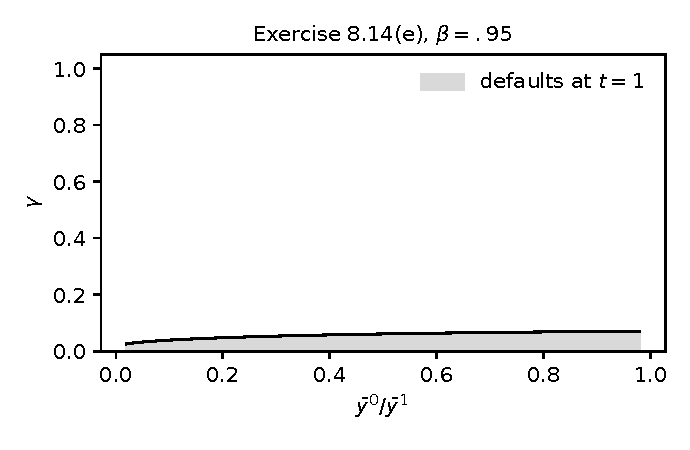
\includegraphics[width=.62\textwidth]{fig/ls08_default.pdf}
\captionof{figure}{Exercise 8.14(e): parameter region in which type 0 defaults at $t=1$ ($\beta=.95$).}
\end{center}
\end{tcolorbox}

%----------------------------------------------------------------------
\subsection{Heterogeneous Beliefs (8.15--8.19)}
%----------------------------------------------------------------------

%------- 8.15 -------
\begin{tcolorbox}[oddbox,title={Exercise 8.15 \quad Diverse beliefs, I}]
\begin{tcolorbox}[questionbox]
pp.~317--318. A pure endowment economy is populated by two consumers. Consumer $i$ has preferences over
history-contingent consumption sequences $\{c^i_t(s^t)\}$ that are ordered by
\[
\sum_{t=0}^\infty\sum_{s^t}\beta^tu(c^i_t(s^t))\pi^i_t(s^t),
\]
where $u(c)=\ln(c)$ and where $\pi^i_t(s^t)$ is a density that consumer $i$ assigns to history $s^t$. The state
space is time invariant. In particular, $s_t\in S=\{0,.5,1\}$ for all $t\ge0$. Only two histories are possible for
$t=0,1,2,\dots$:
\[
\text{history 1}:\ .5,1,1,1,1,\dots\qquad\text{history 2}:\ .5,0,0,0,0,\dots
\]
Consumer 1 assigns probability 1/3 to history 1 and probability 2/3 to history 2, while consumer 2 assigns
probability 2/3 to history 1 and probability 1/3 to history 2. Nature assigns equal probabilities to the two
histories. The endowments of the two consumers are:
\[
y^1_t=s_t,\qquad y^2_t=1-s_t.
\]

\textbf{a.} Define a competitive equilibrium with sequential trading of a complete set of one-period Arrow
securities.

\textbf{b.} Compute a competitive equilibrium with sequential trading of a complete set of one-period Arrow
securities.

\textbf{c.} Is the equilibrium allocation Pareto optimal?
\end{tcolorbox}

\textbf{Solution:}

\textbf{(a)} As in section 8.8.5, with subjective probabilities. Objects: pricing kernels $\tilde Q_t(s_{t+1}|s^t)$;
natural debt limits $A^i_t(s^t)$ (8.8.2); an allocation $\{c^i_t(s^t)\}$ and portfolios $\{\tilde a^i_{t+1}(s_{t+1},s^t)\}$;
initial wealth $\tilde a^i_0=0$. Given kernels and limits, each consumer maximises his subjective expected utility subject to
(8.8.3)--(8.8.4). Markets clear: $c^1+c^2=1$, $\tilde a^1+\tilde a^2=0$. Interior optimality gives
$\tilde Q_t(s_{t+1}|s^t)=\beta\pi^i_t(s^{t+1}|s^t)\,c^i_t(s^t)/c^i_{t+1}(s^{t+1})$ for $i=1,2$.

\textbf{(b)} The aggregate endowment is 1 always. After $t=1$ there is no uncertainty, so within each history
consumption is constant and $\tilde Q=\beta$. At $t=0$ the Euler equations for $s_1=1$ (history 1) and $s_1=0$
(history 2) are
\[
\tilde Q(1)=\beta\tfrac13\frac{c^1_0}{c^1(h_1)}=\beta\tfrac23\frac{c^2_0}{c^2(h_1)},\qquad
\tilde Q(0)=\beta\tfrac23\frac{c^1_0}{c^1(h_2)}=\beta\tfrac13\frac{c^2_0}{c^2(h_2)} .
\]
Let $k=c^1_0/c^2_0$. Then $c^1(h_1)/c^2(h_1)=k/2$ and $c^1(h_2)/c^2(h_2)=2k$, so
$c^1_0=\frac{k}{1+k}$, $c^1(h_1)=\frac{k}{2+k}$, $c^1(h_2)=\frac{2k}{1+2k}$. Equivalently, with time-0 prices
$q_t(h)=\beta^t\pi^1(h)/(\mu_1c^1(h))$ and $\mu_1=1/c^1_0=(1+k)/k$, consumer 1's budget (log utility: the value of
consumption is $1/[\mu_1(1-\beta)]$) reads
\begin{align*}
&\frac{1}{\mu_1(1-\beta)}=.5+\frac{\beta}{1-\beta}\,\frac{1/3}{\mu_1c^1(h_1)}\\
\iff&\frac{1}{1-\beta}=\frac{1+k}{2k}+\frac{\beta(2+k)}{3k(1-\beta)}\\
\iff&6k=3(1+k)(1-\beta)+2\beta(2+k)\iff k(3+\beta)=3+\beta .
\end{align*}
So $k=1$ for every $\beta$, and
\[
\boxed{\begin{gathered}c^1_0=c^2_0=.5;\quad c^1(h_1)=\tfrac13,\ c^2(h_1)=\tfrac23;\quad c^1(h_2)=\tfrac23,\ c^2(h_2)=\tfrac13;\\
\tilde Q_0(1)=\tilde Q_0(0)=\tfrac\beta2,\qquad\tilde Q_t=\beta\ (t\ge1).\end{gathered}}
\]
Holdings $\tilde a=\Upsilon$: $a^1(h_1)=(\tfrac13-1)/(1-\beta)=-\tfrac{2/3}{1-\beta}$ and $a^1(h_2)=\tfrac{2/3}{1-\beta}$,
with $a^2=-a^1$. The t=0 budget: $.5+\tfrac\beta2(a^1(h_1)+a^1(h_2))=.5$. \checkmark{} Each consumer
\emph{bets on his beliefs}. Consumer 1 thinks history 2 is likely, so he buys claims on it and ends up
consuming $2/3$ there, although his endowment there is zero. The natural debt limits (zero for consumer 1 in
$h_2$ and for consumer 2 in $h_1$) do not bind.

\textbf{(c)} Yes, relative to the consumers' own preferences. The allocation satisfies (8.B.2) with $\lambda_1=\lambda_2$:
on $h_1$, $\frac{\pi^2}{\pi^1}\frac{u'(c^2)}{u'(c^1)}=2\cdot\frac{1/3}{2/3}=1$, and likewise on $h_2$. So it solves the
Pareto problem with subjective expected utilities (first welfare theorem). Nature's probabilities play no role in
Pareto optimality. Measured with the true $(\frac12,\frac12)$, each consumer's consumption is risky: that is the price
of disagreement.

\begin{tcolorbox}[databox]
\texttt{brentq} on consumer 1's budget gives $k=1$ for $\beta\in\{.5,.9,.95\}$. With $\beta=.95$: both consumers'
Euler equations give $\tilde Q_0=(.475,.475)$ and $a^1=(-13.333,\ 13.333)$.
\end{tcolorbox}
\end{tcolorbox}

%------- 8.16 -------
\begin{tcolorbox}[evenbox,title={Exercise 8.16 \quad Diverse beliefs, II}]
\begin{tcolorbox}[questionbox]
pp.~318--319. Consider the following $I$ person pure endowment economy. There is a state variable $s_t\in S$
for all $t\ge0$. Let $s^t$ denote a history of $s$ from 0 to $t$. The time $t$ aggregate endowment is a
function of the history, so $Y_t=Y_t(s^t)$. Agent $i$ attaches a personal probability of $\pi^i_t(s^t)$ to history
$s^t$. The history $s^t$ is observed by all $I$ people at time $t$. Assume that for all $i$, $\pi^i_t(s_t)>0$ if and
only if $\pi^1_t(s_t)>0$ (so the consumers agree about which histories have positive probability). Consumer
$i$ ranks consumption plans $c^i_t(s^t)$ that are measurable functions of histories via the expected utility
functional
\[
\sum_{t=0}^\infty\sum_{s^t}\beta^t\ln(c^i_t(s^t))\pi^i_t(s^t) \tag{1}
\]
The ownership structure of the economy is not yet determined.

A planner puts positive Pareto weights $\lambda_i>0$ on consumers $i=1,\dots,I$ and solves a time 0 Pareto
problem that respects each consumer's preferences as represented by (1).

\textbf{a.} Show how to solve for a Pareto optimal allocation. Display an expression for $c^i_t(s^t)$ as a
function of $Y_t(s^t)$ and other pertinent variables.

\textbf{b.} Under what circumstances does the Pareto plan imply complete risk-sharing among the $I$
consumers?

\textbf{c.} Under what circumstances does the Pareto plan imply an allocation that is not history
dependent? By `not history dependent', we mean that $Y_t(s^t)=Y_t(\tilde s^t)$ would imply the same
allocation at time $t$?

\textbf{d.} For a given set of Pareto weights, find an associated equilibrium price vector and an initial
distribution of wealth among the $I$ consumers that makes the Pareto allocation be the allocation
associated with a competitive equilibrium with time 0 trading of history-contingent claims on consumption.

\textbf{e.} Find a formula for the equilibrium price vector in terms of equilibrium quantities and the beliefs of
consumers.

\textbf{f.} Suppose that $I=2$. Show that as $\lambda_2/\lambda_1\to+\infty$, the planner would distribute initial
wealth in a way that makes consumer 2's beliefs more and more influential in determining equilibrium
prices.
\end{tcolorbox}

\textbf{Solution:}

\textbf{(a)} Lagrangian:
$\mathcal L=\sum_t\sum_{s^t}\big\{\sum_i\lambda_i\beta^t\ln c^i_t(s^t)\pi^i_t(s^t)+\theta_t(s^t)[Y_t(s^t)-\sum_ic^i_t(s^t)]\big\}$.
FOC: $\lambda_i\beta^t\pi^i_t(s^t)/c^i_t(s^t)=\theta_t(s^t)$, so $c^i_t=\lambda_i\beta^t\pi^i_t/\theta_t$. Summing over $i$ and using
feasibility, $\theta_t(s^t)=\beta^t\sum_j\lambda_j\pi^j_t(s^t)/Y_t(s^t)$. Hence
\[
\boxed{c^i_t(s^t)=\frac{\lambda_i\pi^i_t(s^t)}{\sum_{j=1}^I\lambda_j\pi^j_t(s^t)}\,Y_t(s^t).}
\]
Shares are weighted by Pareto weight times the consumer's probability of the history (likelihood ratios, as in (8.B.2)).

\textbf{(b)} Complete risk sharing means that each consumer's share $c^i_t/Y_t$ is the same across all histories.
The share is $\lambda_iL^i_t/\sum_j\lambda_jL^j_t$ with $L^j_t=\pi^j_t/\pi^1_t$. It is constant across $s^t$ iff each
$L^j_t(s^t)$ is constant across $s^t$. Since $\sum_{s^t}\pi^j_t=\sum_{s^t}\pi^1_t=1$, the constant must be 1. So there is
complete risk sharing iff \textbf{beliefs are common}, $\pi^i_t=\pi^1_t$ for all $i$ (on histories with positive
probability). The shares are then $\lambda_i/\sum_j\lambda_j$.

\textbf{(c)} $c^i_t(s^t)$ depends on $s^t$ only through $Y_t(s^t)$ iff every likelihood ratio $\pi^j_t(s^t)/\pi^1_t(s^t)$
is a function of $(t,Y_t(s^t))$ only. Sufficiency is clear from (a). For necessity, $c^j_t/c^1_t=\lambda_jL^j_t/\lambda_1$
must then be a function of $Y_t$. Common beliefs are the leading case. Disagreement is harmless only about events
that the aggregate endowment reveals.

\textbf{(d)} Prices $=$ normalised multipliers (section 8.5.2), with $q^0_0(s_0)=1$ and $\pi^j_0(s_0)=1$:
\[
q^0_t(s^t)=\frac{\theta_t(s^t)}{\theta_0(s_0)}=\beta^t\frac{Y_0}{Y_t(s^t)}\sum_j\omega_j\pi^j_t(s^t),\qquad
\omega_j\equiv\frac{\lambda_j}{\sum_k\lambda_k}.
\]
Consumer $i$'s consumption is worth
$\sum_t\sum_{s^t}q^0_tc^i_t=\sum_t\beta^tY_0\omega_i\sum_{s^t}\pi^i_t=\omega_iY_0/(1-\beta)$, and total wealth is
$\sum_t\sum_{s^t}q^0_tY_t=Y_0/(1-\beta)$. An initial distribution that supports the plan gives consumer $i$ wealth
$\omega_iY_0/(1-\beta)$. For example, endow consumer $i$ with the fraction $\omega_i=\lambda_i/\sum_k\lambda_k$ of the
aggregate endowment in every history. Each consumer's FOC $\beta^t\pi^i_t/c^i_t=\mu_iq^0_t$ holds with
$\mu_i=1/c^i_0$.

\textbf{(e)} From $\beta^t\pi^i_t/c^i_t=q^0_t/c^i_0$, we get $q^0_tc^i_t=\beta^tc^i_0\pi^i_t$. Summing over $i$:
\[
\boxed{q^0_t(s^t)=\beta^t\,\frac{1}{Y_t(s^t)}\sum_ic^i_0\,\pi^i_t(s^t)=\beta^t\frac{Y_0}{Y_t(s^t)}\sum_i\frac{c^i_0}{Y_0}\,\pi^i_t(s^t).}
\]
This is the marginal utility of the aggregate endowment times a consumption-share-weighted average of beliefs.

\textbf{(f)} With $I=2$, $\omega_2=\frac{\lambda_2/\lambda_1}{1+\lambda_2/\lambda_1}\to1$, so consumer 2's initial wealth share
$\to1$ and $q^0_t\to\beta^t(Y_0/Y_t)\pi^2_t(s^t)$: prices are those of an economy in which everyone holds consumer
2's beliefs.

\begin{tcolorbox}[databox]
Random example ($I=3$, four date-1 nodes, $\lambda=(1,2,.5)$, $\beta=.9$): SLSQP on the planner's node-by-node problem
reproduces (a); every consumer's FOC holds at the prices of (e).
\end{tcolorbox}
\end{tcolorbox}

%------- 8.17 -------
\begin{tcolorbox}[oddbox,title={Exercise 8.17 \quad Diverse beliefs, III}]
\begin{tcolorbox}[questionbox]
pp.~319--320. An economy consists of two consumers named $i=1,2$. Each consumer evaluates streams of a
single nonstorable consumption good according to
\[
\sum_{t=0}^\infty\sum_{s^t}\beta^t\ln[c^i_t(s^t)]\pi^i_t(s^t).
\]
Here $\pi^i_t(s^t)$ is consumer $i$'s subjective probability over history $s^t$. A feasible allocation satisfies
$\sum_ic^i_t(s^t)\le\sum_iy^i(s_t)$ for all $t\ge0$ and for all $s^t$. The consumers' endowments of the one good are
functions of a state variable $s_t\in\mathbf S=\{0,1,2\}$. In truth, $s_t$ is described by a time invariant
Markov chain with initial distribution $\pi_0=[\,0\ \ 1\ \ 0\,]'$ and transition density defined by the
stochastic matrix
\[
P=\begin{bmatrix}1&0&0\\.5&0&.5\\0&0&1\end{bmatrix}
\]
where $P_{ij}=\mathrm{Prob}[s_{t+1}=j-1|s_t=i-1]$ for $i=1,2,3$ and $j=1,2,3$. The endowments of the two
consumers are
\[
y^1_t=s_t/2,\qquad y^2_t=1-s_t/2.
\]
In part I, both consumers know the true probabilities over histories $s^t$ (i.e., they know both $\pi_0$ and
$P$). In part II, the two consumers have different subjective probabilities.

\textbf{Part I:} Assume that both consumers know $(\pi_0,P)$, so that $\pi^1_t(s^t)=\pi^2_t(s^t)$ for all $t\ge0$ for
all $s^t$.

\textbf{a.} Show how to deduce $\pi^i_t(s^t)$ from $(\pi_0,P)$.

\textbf{b.} Define a competitive equilibrium with sequential trading of Arrow securities.

\textbf{c.} Compute a competitive equilibrium with sequential trading of Arrow securities.

\textbf{d.} By hand, simulate the economy. In particular, for every possible realization of the histories $s^t$,
describe time series of $c^1_t,c^2_t$ and the wealth levels for the two consumers.

\textbf{Part II:} Now assume that while consumer 1 knows $(\pi_0,P)$, consumer 2 knows $\pi_0$ but thinks
that $P$ is
\[
\hat P=\begin{bmatrix}1&0&0\\.4&0&.6\\0&0&1\end{bmatrix}.
\]

\textbf{e.} Deduce $\pi^2_t(s^t)$ from $(\pi_0,\hat P)$ for all $t\ge0$ for all $s^t$.

\textbf{f.} Formulate and solve a Pareto problem for this economy.

\textbf{g.} Define an equilibrium with time 0 trading of a complete set of Arrow-Debreu history-contingent
securities.

\textbf{h.} Compute an equilibrium with time 0 trading of a complete set of Arrow-Debreu history-contingent
securities.

\textbf{i.} Compute an equilibrium with sequential trading of Arrow securities. For every possible realization
of $s^t$ for all $t\ge0$, please describe time series of $c^1_t,c^2_t$ and the wealth levels for the two
consumers.
\end{tcolorbox}

\textbf{Solution:}

\textbf{Part I.} \textbf{(a)} $\pi_t(s^t)=\pi_0(s_0)\prod_{k=1}^tP(s_k|s_{k-1})$. Here $s_0=1$ surely. For $t\ge1$,
$\pi_t(1,0,\dots,0)=\pi_t(1,2,\dots,2)=.5$, and every other history has probability zero.
\textbf{(b)--(d)} This is Exercise 8.13 with $u=\ln$. The definition is 8.13(a) with $u=\ln$. Solution:
$Q(s'|s)=\beta P(s'|s)$, $c^1=c^2=.5$ in every history. Holdings: consumer 1 has
$a^1=+.5/(1-\beta)$ on $(1,0,0,\dots)$ and $-.5/(1-\beta)$ on $(1,2,2,\dots)$ for $t\ge1$, and zero at $t=0$;
$a^2=-a^1$. The table of 8.13(c) applies unchanged.

\textbf{Part II.} \textbf{(e)} $\pi^2_0(1)=1$; for $t\ge1$, $\pi^2_t(1,0,\dots,0)=.4$ and $\pi^2_t(1,2,\dots,2)=.6$;
zero otherwise.

\textbf{(f)} $\max\ \lambda U_1+(1-\lambda)U_2$ s.t.\ $c^1+c^2\le1$. By 8.16(a),
$c^1_t=\lambda\pi^1_t/(\lambda\pi^1_t+(1-\lambda)\pi^2_t)$:
\[
c^1_0=\lambda,\qquad c^1(\text{path }0)=\frac{.5\lambda}{.5\lambda+.4(1-\lambda)}=\frac{.5\lambda}{.4+.1\lambda},\qquad
c^1(\text{path }2)=\frac{.5\lambda}{.6-.1\lambda},
\]
with $c^2=1-c^1$, constant along each path for $t\ge1$.

\textbf{(g)} Prices $\{q^0_t(s^t)\}$ and an allocation such that each consumer maximises his \emph{subjective}
expected utility subject to $\sum_t\sum_{s^t}q^0_t(c^i_t-y^i_t)\le0$, and $c^1+c^2=1$.

\textbf{(h)} By 8.16(d) with $Y\equiv1$ and weights $(\lambda,1-\lambda)$:
$q^0_t(\text{path }0)=\beta^t(.4+.1\lambda)$ and $q^0_t(\text{path }2)=\beta^t(.6-.1\lambda)$ for $t\ge1$. Consumer 1's
wealth is $\lambda/(1-\beta)$ (8.16(d)). His endowment is $.5$ at $t=0$, $0$ on path 0, and $1$ on path 2:
\[
\frac{\lambda}{1-\beta}=.5+\frac{\beta}{1-\beta}(.6-.1\lambda)\iff\lambda(1+.1\beta)=.5+.1\beta\iff
\boxed{\lambda=\frac{.5+.1\beta}{1+.1\beta}>\frac12 .}
\]
Consumer 2 is optimistic about path 2, where consumer 1 owns everything. That bids up the value of consumer 1's
endowment and makes him richer. Yet consumer 1 consumes more on path 0, which he thinks more likely than consumer 2
does.

\textbf{(i)} Kernel at $s=1$: $Q(0|1)=\beta(.4+.1\lambda)$, $Q(2|1)=\beta(.6-.1\lambda)$; $Q(s|s)=\beta$ for $s\in\{0,2\}$.
Consumption as in (f). Wealth: $a^i_0=0$. For $t\ge1$, $a^1=c^1(\text{path }0)/(1-\beta)$ on path 0 and
$a^1=[c^1(\text{path }2)-1]/(1-\beta)$ on path 2; $a^2=-a^1$. At $t=0$ consumer 1 consumes $\lambda>.5$, selling claims
on path 2 and buying claims on path 0.

\begin{tcolorbox}[databox]
$\beta=.95$ (not given): $\lambda=.543379$; $Q(0|1)=.431621$, $Q(2|1)=.518379$; $c^1=(.59799,\ .49791)$ on paths
$(0,2)$; $a^1=(11.9598,\ -10.0418)$. \texttt{brentq} on the budget recovers $\lambda$. Both Euler equations and
both $t=0$ Arrow budgets hold.
\end{tcolorbox}
\end{tcolorbox}

%------- 8.18 -------
\begin{tcolorbox}[evenbox,title={Exercise 8.18 \quad Diverse beliefs, IV}]
\begin{tcolorbox}[questionbox]
pp.~320--321. A pure exchange economy is populated by two consumers. Consumer $i$ has preferences over
history-contingent consumption sequences $\{c^i_t(s^t)\}$ that are ordered by
\[
\sum_{t=0}^\infty\sum_{s^t}\beta^tu(c^i_t(s^t))\pi^i_t(s^t),
\]
where $u(c)=\ln(c)$, $\beta\in(0,1)$, and $\pi^i_t(s^t)$ is a density that consumer $i$ assigns to history $s^t$.
The state space is time invariant. In particular, $s_t\in S=\{0,.5,1\}$ for all $t\ge0$. Only two histories are
possible for $t=0,1,2,\dots$:
\[
\text{history 1}:\ .5,1,1,1,1,\dots\qquad\text{history 2}:\ .5,0,0,0,0,\dots
\]
Consumer 1 assigns probability 1 to history 1 and probability 0 to history 2, while consumer 2 assigns
probability 0 to history 1 and probability 1 to history 2. Nature assigns equal probabilities to the two
histories. The endowments of the two consumers are:
\[
y^1_t=s_t,\qquad y^2_t=1-s_t.
\]

\textbf{a.} Formulate and solve a Pareto problem for this economy.

\textbf{b.} Define a competitive equilibrium with sequential trading of a complete set of one-period Arrow
securities.

\textbf{c.} Does a competitive equilibrium with sequential trading of a complete set of one-period Arrow
securities exist for this economy? If it does, compute it. If it does not, explain why.
\end{tcolorbox}

\textbf{Solution:}

\emph{Convention.} Utility terms on histories with subjective probability zero contribute nothing
($0\cdot\ln0=0$). Consumption there is only restricted by $c\ge0$ and the budget.

\textbf{(a)} $\max\ \lambda\sum_t\sum_{s^t}\beta^t\ln c^1_t\,\pi^1_t+(1-\lambda)\sum_t\sum_{s^t}\beta^t\ln c^2_t\,\pi^2_t$
s.t.\ $c^1_t+c^2_t\le1$. At $t=0$ both have probability one: $\lambda/c^1_0=(1-\lambda)/c^2_0$, so $c^1_0=\lambda$. For
$t\ge1$ on history 1 only consumer 1's utility counts, so $c^1=1$, $c^2=0$. On history 2, $c^1=0$, $c^2=1$. This is
the formula $c^1_t=\lambda\pi^1_t/(\lambda\pi^1_t+(1-\lambda)\pi^2_t)$ of 8.16(a). Each consumer gets everything in the
history he believes in.

\textbf{(b)} As in 8.15(a): kernels, natural debt limits $A^i_t(s^t)$, allocation and portfolios with $\tilde a^i_0=0$.
Each consumer solves (8.8.3)--(8.8.4) under his own beliefs, and markets clear.

\textbf{(c)} \textbf{It exists, and it involves no trade.} The endowment gives consumer 1 $.5$ at $t=0$, 1 forever on
history 1 and 0 on history 2. That is exactly the Pareto allocation with $\lambda=.5$. Prices at $t=0$: consumer 1's
Euler equation on history 1 gives $\tilde Q(s_1{=}1)=\beta\cdot1\cdot\frac{.5}{1}=.5\beta$; consumer 2's on history 2
gives $\tilde Q(s_1{=}0)=.5\beta$; afterwards $\tilde Q=\beta$. At these prices consumer 1 is content with zero
holdings of claims on history 1. He would like to \emph{sell} claims on history 2 (positive price, zero value to
him), but his natural debt limit there is $A^1(\text{history 2})=0$: his endowment is zero forever, so
$\tilde a^1(0)\ge0$ binds. Symmetrically for consumer 2 on history 1. Nobody trades. The allocation is Pareto
optimal. The natural debt limits \emph{bind}, contrary to section 8.8.4: the Inada argument needs every history
to have positive subjective probability.
\end{tcolorbox}

%------- 8.19 -------
\begin{tcolorbox}[oddbox,title={Exercise 8.19 \quad Diverse beliefs, V}]
\begin{tcolorbox}[questionbox]
pp.~321--322. A pure exchange economy is populated by two consumers. Consumer $i$ has preferences over
history-contingent consumption sequences $\{c^i_t(s^t)\}$ that are ordered by
$\sum_{t=0}^\infty\sum_{s^t}\beta^tu(c^i_t(s^t))\pi^i_t(s^t)$, where $u(c)=\ln(c)$, $\beta\in(0,1)$, and $\pi^i_t(s^t)$ is
a density that consumer $i$ assigns to history $s^t$. The state space is time invariant. In particular,
$s_t\in S=\{0,.5,1\}$ for all $t\ge0$. Only two histories are possible for $t=0,1,2,\dots$: history 1:
$.5,1,1,1,1,\dots$; history 2: $.5,0,0,0,0,\dots$. Consumer 1 assigns probability 1 to history 1 and
probability 0 to history 2, while consumer 2 assigns probability 0 to history 1 and probability 1 to history 2.
Nature assigns equal probabilities to the two histories. The endowments of the two consumers are:
\[
y^1_t=1-s_t,\qquad y^2_t=s_t.
\]

\textbf{a.} Formulate and solve a Pareto problem for this economy.

\textbf{b.} Define a competitive equilibrium with sequential trading of a complete set of one-period Arrow
securities.

\textbf{c.} Does a competitive equilibrium with sequential trading of a complete set of one-period Arrow
securities exist for this economy? If it does, compute it. If it does not, explain why.
\end{tcolorbox}

\textbf{Solution:}

\textbf{(a)} Preferences are those of 8.18, so the Pareto set is the same: $c^1_0=\lambda$, $c^1=1$ on history 1 and $0$
on history 2 ($t\ge1$), $c^2=1-c^1$.

\textbf{(b)} As in 8.18(b).

\textbf{(c)} \textbf{It exists, with maximal trade.} Now each consumer owns everything in the history he rules out:
consumer 1 has 1 forever on history 2 and 0 on history 1. Natural debt limits:
$A^1(\text{history 2})=A^2(\text{history 1})=1/(1-\beta)$ (claims priced at $\tilde Q=\beta$ after $t=1$), and
$A^1(\text{history 1})=A^2(\text{history 2})=0$. Guess symmetric prices $\tilde Q(s_1{=}1)=\tilde Q(s_1{=}0)=q$.
Consumer 1 sells history-2 claims up to his limit, $\tilde a^1(0)=-1/(1-\beta)$, and uses the proceeds to buy
$\tilde a^1(1)=1/(1-\beta)$. The cost is $q[1/(1-\beta)-1/(1-\beta)]=0$, so $c^1_0=.5$. His Euler equation on history 1:
$q=\beta\cdot1\cdot\frac{c^1_0}{c^1(h_1)}$. With $c^1(h_1)=1$ this gives $q=.5\beta$. For $t\ge1$ on history 1: he holds
$1/(1-\beta)$, has endowment 0, and consumes 1, since $1+\beta\cdot\frac1{1-\beta}=0+\frac1{1-\beta}$. On history 2 he owes
$1/(1-\beta)$, pays his whole endowment 1 each period, and consumes 0. Consumer 2 is symmetric; the markets
clear. The allocation is the Pareto allocation with $\lambda=.5$, the same as in 8.18, but it is reached by trade in
which each consumer borrows \emph{exactly up to} his natural debt limit in the history he rules out.

\emph{Comparison.} In both 8.18 and 8.19 an equilibrium exists because $c\ge0$ is allowed and zero-probability
histories carry no utility weight. What differs is who owns what. When the ``impossible'' history is realised,
the losing consumer consumes zero forever, and his beliefs cannot be revised by Bayes' rule. Equilibrium relies
on debts that are enforced at the natural limit.

\begin{tcolorbox}[databox]
$\beta=.95$: $\tilde Q_0=(.475,.475)$; the notebook verifies the $t=0$ budget, the roll-over budgets on both
histories, and that the debt limit binds.
\end{tcolorbox}
\end{tcolorbox}

%----------------------------------------------------------------------
\subsection{Risk-Free Bonds, Entropy and Beliefs Again (8.20--8.23)}
%----------------------------------------------------------------------

%------- 8.20 -------
\begin{tcolorbox}[evenbox,title={Exercise 8.20 \quad Risk-free bonds}]
\begin{tcolorbox}[questionbox]
pp.~322--323. An economy consists of a single representative consumer who ranks streams of a single
nonstorable consumption good according to $\sum_{t=0}^\infty\sum_{s^t}\beta^t\ln[c_t(s^t)]\pi_t(s^t)$. Here $\pi_t(s^t)$
is the subjective probability that the consumer attaches to a history $s^t$ of a Markov state $s_t$, where
$s_t\in\{1,2\}$. Assume that the subjective probability $\pi_t(s^t)$ equals the objective probability. Feasibility
for this pure endowment economy is expressed by the condition $c_t\le y_t$, where $y_t$ is the endowment at
time $t$. The endowment is exogenous and governed by
\[
y_{t+1}=\lambda_{t+1}\lambda_t\cdots\lambda_1y_0
\]
for $t\ge0$ where $y_0>0$. Here $\lambda_t$ is a function of the Markov state $s_t$. Assume that $\lambda_t=1$ when
$s_t=1$ and $\lambda_t=1+\zeta$ when $s_t=2$, where $\zeta>0$. States $s^t=[s_t,\dots,s_0]$ are known at time $t$,
but future states are not. The state $s_t$ is described by a time invariant Markov chain with initial
probability distribution $\pi_0=[\,1\ \ 0\,]'$ and transition density defined by the stochastic matrix
\[
P=\begin{bmatrix}P_{11}&P_{12}\\P_{21}&P_{22}\end{bmatrix}
\]
where $P_{ij}=\mathrm{Prob}[s_{t+1}=j|s_t=i]$ for $i=1,2$ and $j=1,2$. Assume that $P_{ij}\ge0$ for all pairs $(i,j)$.

\textbf{a.} Show how to deduce $\pi_t(s^t)$ from $(\pi_0,P)$.

\textbf{b.} Define a competitive equilibrium with sequential trading of Arrow securities.

\textbf{c.} Compute a competitive equilibrium with sequential trading of Arrow securities.

\textbf{d.} Let $p^b_t$ be the time $t$ price of a risk-free claim to one unit of consumption at time $t+1$. Define a
competitive equilibrium with sequential trading of risk-free claims to consumption one period ahead.

\textbf{e.} Let $R_t=(p^b_t)^{-1}$ be the one-period risk-free gross interest rate. Give a formula for $R_t$ and
tell how it depends on the history $s^t$.

\textbf{f.} Suppose that $\beta=.95$, $\zeta=.02$ and $P=\begin{bmatrix}1&0\\.5&.5\end{bmatrix}$. Please compute $R_t$
when $s_t=1$. Then compute $R_t$ when $s_t=2$.

\textbf{g.} What parts of your answers depend on assuming that the subjective probability $\pi_t(s^t)$ equals
the objective probability?
\end{tcolorbox}

\textbf{Solution:}

\textbf{(a)} $\pi_t(s^t)=\pi_0(s_0)P_{s_0s_1}P_{s_1s_2}\cdots P_{s_{t-1}s_t}$; $\pi_0=(1,0)$ means $s_0=1$.

\textbf{(b)} A kernel $\tilde Q_t(s_{t+1}|s^t)$, natural debt limits $A_t(s^t)$, an allocation $c_t(s^t)$ and portfolios
$\tilde a_{t+1}(s_{t+1},s^t)$ with $\tilde a_0=0$. Given the kernel, the consumer maximises utility subject to (8.8.3)--(8.8.4).
Markets clear: $c_t=y_t$, $\tilde a_{t+1}=0$ (zero net supply).

\textbf{(c)} $c_t=y_t$, $\tilde a\equiv0$, and from (8.8.6) with $u'(c)=1/c$:
\[
\tilde Q_t(s_{t+1}|s^t)=\beta P_{s_ts_{t+1}}\frac{y_t}{y_{t+1}}=\frac{\beta P_{s_ts_{t+1}}}{\lambda(s_{t+1})}\equiv Q(s_{t+1}|s_t).
\]
Natural debt limits: with log utility $q^t_\tau y_\tau=\beta^{\tau-t}\pi\,y_t$, so $A_t=y_t/(1-\beta)$.

\textbf{(d)} A price $p^b_t(s^t)$, an allocation, and bond holdings $b_{t+1}$ such that the consumer maximises
utility s.t.\ $c_t+p^b_tb_{t+1}\le y_t+b_t$, $b_0=0$, and a debt limit that rules out Ponzi schemes; and markets
clear: $c_t=y_t$, $b_{t+1}=0$.

\textbf{(e)} The Euler equation at $b=0$: $p^b_t=\beta E_t[y_t/y_{t+1}]=\sum_{s'}Q(s'|s_t)$, so
\[
\boxed{R_t=\Big[\beta\sum_{j}\frac{P_{s_tj}}{\lambda(j)}\Big]^{-1},}
\]
which depends on the history only through the current state $s_t$.

\textbf{(f)} $s_t=1$: $R=1/(.95\cdot1)=1.052632$. $s_t=2$: $R=1/[.95(.5+.5/1.02)]=1.063054$. With $\pi_0=(1,0)$ and
$P_{11}=1$, state 2 is never visited, so $R(2)$ is an off-path value. The economy stays in state 1 with zero growth
and $R=1/\beta$.

\textbf{(g)} None of the equilibrium conditions uses the objective probabilities. The allocation ($c=y$) does not
depend on probabilities at all. Prices $Q$, $p^b$ and $R$ are computed from the consumer's \emph{subjective}
$P$; with a different subjective matrix the same formulas hold with that matrix. What depends on
subjective $=$ objective is the interpretation of prices as expectations under the data-generating process:
average realised returns, the frequency with which $R(2)$ is observed, and statistical tests of asset-pricing
Euler equations.
\end{tcolorbox}

%------- 8.21 -------
\begin{tcolorbox}[oddbox,title={Exercise 8.21 \quad Entropy}]
\begin{tcolorbox}[questionbox]
p.~323. Let $\tilde f(s)$ and $f(s)$ be two alternative probability density functions for a random variable $s$.
Define the relative entropy of $f$ with respect to $\tilde f$ by
\[
\ent(f,\tilde f)=\int\log\Big(\frac{\tilde f(s)}{f(s)}\Big)\tilde f(s)ds=\int\log\Big(\frac{\tilde f(s)}{f(s)}\Big)\Big(\frac{\tilde f(s)}{f(s)}\Big)f(s)ds.
\]
Prove that $\ent(f,\tilde f)\ge0$ and that $\ent(\tilde f,\tilde f)=0$.

\textbf{Hint 1:} Define $m(s)=\big(\frac{\tilde f(s)}{f(s)}\big)$ and express entropy as $\int m(s)\log m(s)f(s)ds$.

\textbf{Hint 2:} Verify that $m\log m\ge m-1$.

\textbf{Hint 3:} Verify that $\int m(s)f(s)=1$.
\end{tcolorbox}

\textbf{Solution:}

Assume $\tilde f\ll f$ ($f>0$ wherever $\tilde f>0$), so $m=\tilde f/f$ is well defined; set $0\log0=0$.

\emph{Hint 1.} $\ent(f,\tilde f)=\int\log m\cdot m\,f\,ds=\int m\log m\,f\,ds$.

\emph{Hint 2.} Let $g(m)=m\log m-m+1$ on $m\ge0$. Then $g(1)=0$, $g'(m)=\log m$ ($<0$ for $m<1$, $>0$ for $m>1$), and
$g''(m)=1/m>0$. So $g$ has its unique minimum $0$ at $m=1$, and $g\ge0$; at $m=0$, $g(0)=1>0$.

\emph{Hint 3.} $\int mf\,ds=\int\tilde f\,ds=1$.

\emph{Proof.} $\ent(f,\tilde f)=\int m\log m\,f\,ds\ge\int(m-1)f\,ds=1-1=0$. Equality requires $g(m(s))=0$
$f$-almost everywhere, i.e.\ $\tilde f=f$ a.e. For $f=\tilde f$, $m\equiv1$ and $\log1=0$, so
$\ent(\tilde f,\tilde f)=0$.

\begin{tcolorbox}[databox]
$m\log m\ge m-1$ on a grid of $2\times10^5$ points in $(0,50]$; $\ent\ge0$ and $\int mf=1$ on 1000 random pairs of
discrete densities.
\end{tcolorbox}
\end{tcolorbox}

%------- 8.22 -------
\begin{tcolorbox}[evenbox,title={Exercise 8.22 \quad Heterogeneous beliefs again}]
\begin{tcolorbox}[questionbox]
pp.~323--324. Consider an example of the heterogeneous beliefs economy described in Appendix B of this
chapter. Suppose that $S=\{0,1\}$, $I=2$, and that agent $i$ believes that $s_t$ is independently and
identically distributed with $\mathrm{Prob}(s_t=0)=\alpha_i$. Assume that $u_i(c^i_t)=\log c^i_t$ for both
consumers. The aggregate endowment is $y_t(s^t)=1-.5s_t$. Feasibility requires $c^1_t+c^2_t\le y_t(s^t)$. A
time 0 Pareto planner puts weight $\lambda\in(0,1)$ on consumer 1 and weight $(1-\lambda)$ on consumer 2.
Suppose that $\{s_t\}_{t=1}^\infty$ is truly independently and identically distributed with
$\mathrm{Prob}(s_t=0)=\tilde\alpha$. Assume that $I=2$, $\alpha_2=\tilde\alpha$, $\alpha_1\ne\tilde\alpha$, so that consumer 2
knows the true distribution, while consumer 1 does not.

\textbf{a.} Let $L^2_t(s^t)=\frac{\pi^2_t(s^t)}{\pi^1_t(s^t)}$. Show that a Pareto optimal allocation satisfies
\[
c^2_t(s^t)=\Big[\frac{(1-\lambda)L^2(s^t)}{\lambda+(1-\lambda)L^2_t(s^t)}\Big]y_t(s^t).
\]

\textbf{b.} Find a formula for the price $\tilde Q(s_{t+1}|s^t)$ of Arrow securities.

\textbf{c.} State assumptions under which you can show that
\[
\tilde Q_t(s_{t+1}|s^t)\to\beta\Big(\frac{y_t(s_t)}{y_{t+1}(s_{t+1})}\Big)\pi^2_t(s_{t+1}|s^t),
\]
as $t\to+\infty$ in some sense. Describe the sense in which what you claim is true.

\textbf{d.} Use your findings from part \textbf{c} to argue that the ``tail'' of the economy resembles a
representative consumer economy.
\end{tcolorbox}

\textbf{Solution:}

\textbf{(a)} FOC (8.B.2) with $\lambda_1=\lambda$, $\lambda_2=1-\lambda$, $u'=1/c$:
$\lambda\beta^t\pi^1_t/c^1_t=(1-\lambda)\beta^t\pi^2_t/c^2_t$, so $c^1_t=c^2_t\,\lambda/[(1-\lambda)L_t]$. Feasibility
$c^1_t+c^2_t=y_t$ gives $c^2_t\big[1+\frac{\lambda}{(1-\lambda)L_t}\big]=y_t$, which is the stated formula.
\checkmark

\textbf{(b)} Use consumer 2's Euler equation (8.8.6), $\tilde Q=\beta\pi^2(s')c^2_t/c^2_{t+1}$, with
$L_{t+1}=L_t\,\ell(s')$, $\ell(s')=\pi^2(s')/\pi^1(s')$ (i.i.d.\ beliefs):
\[
\frac{c^2_t}{c^2_{t+1}}=\frac{y_t}{y_{t+1}}\frac{L_t}{L_{t+1}}\frac{\lambda+(1-\lambda)L_{t+1}}{\lambda+(1-\lambda)L_t}
\]
so that
\[
\boxed{\tilde Q(s_{t+1}|s^t)=\beta\frac{y_t}{y_{t+1}}\,\frac{\lambda\pi^1(s_{t+1})+(1-\lambda)L_t\,\pi^2(s_{t+1})}{\lambda+(1-\lambda)L_t}}
\]
using $\pi^2(s')L_t/L_{t+1}=\pi^1(s')$. Prices use a consumption-share-weighted average of beliefs, with weight
$w_t=\lambda/(\lambda+(1-\lambda)L_t)=c^1_t/y_t$ on consumer 1's beliefs.

\textbf{(c)} Assumptions: $s_t$ is i.i.d.\ under the truth with $\alpha_2=\tilde\alpha\in(0,1)$; $\alpha_1\in(0,1)$ and
$\alpha_1\ne\tilde\alpha$ (so both consumers give positive probability to both states and $\log\ell$ is finite);
$\lambda\in(0,1)$. Then $\log L_t=\sum_{\tau}\log\ell(s_\tau)$ is a sum of i.i.d.\ terms with true mean
$\ent(\pi^2,\pi^1)=\sum_s\pi^2(s)\log[\pi^2(s)/\pi^1(s)]>0$ (8.21, strict since $\pi^1\ne\pi^2$). By the strong law of
large numbers $\frac1t\log L_t\to\ent(\pi^2,\pi^1)>0$ almost surely, so $L_t\to\infty$ and $w_t\to0$ a.s. Hence, for
each $s_{t+1}$,
\[
\tilde Q(s_{t+1}|s^t)-\beta\frac{y_t}{y_{t+1}}\pi^2(s_{t+1})=\beta\frac{y_t}{y_{t+1}}\,w_t\,[\pi^1(s_{t+1})-\pi^2(s_{t+1})]\to0
\]
\emph{almost surely under the true probability measure}: along almost every sample path, not uniformly, and not
along the zero-probability paths on which consumer 1's beliefs look better. The gap shrinks geometrically,
$w_t\approx\frac{\lambda}{1-\lambda}e^{-t\,\ent(\pi^2,\pi^1)}$.

\textbf{(d)} Along almost every path $c^1_t/y_t=w_t\to0$ and $c^2_t/y_t\to1$. The Arrow prices converge to
$\beta\pi^2(s')y_t/y_{t+1}$, the kernel of a representative consumer with log utility and \emph{correct} beliefs
who consumes the aggregate endowment. So the tail of the economy is a representative-agent, rational-expectations
economy: the market selects for accurate beliefs (Friedman's conjecture, Blume--Easley).

\begin{tcolorbox}[databox]
Illustration $\tilde\alpha=\alpha_2=.5$, $\alpha_1=.7$, $y=(1,.5)$, $\lambda=.5$, $\beta=.95$, five simulated paths of
3000 periods: the formula in (b) equals consumer 2's Euler equation, $\frac1t\log L_t$ is within $.03$ of
$\ent(\pi^2,\pi^1)=.08718$, and the price gap at $t=3000$ is below $10^{-10}$ (figure).
\end{tcolorbox}

\begin{center}
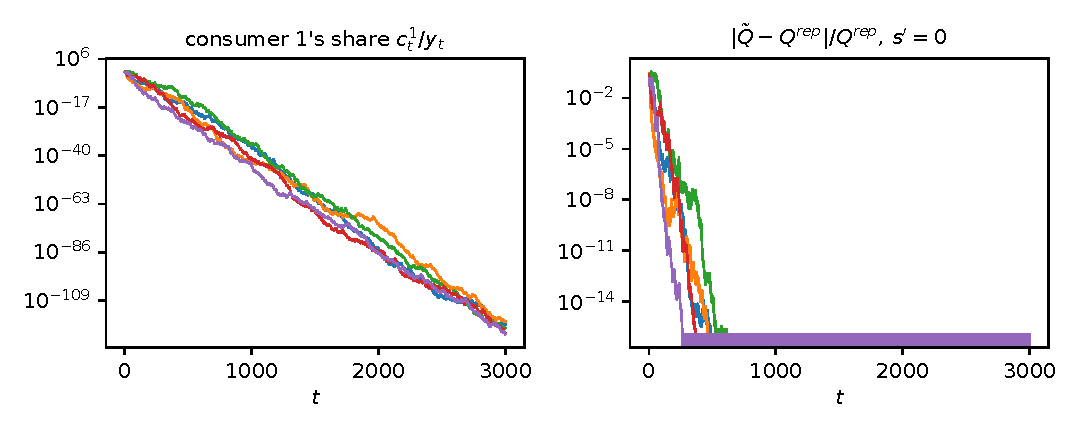
\includegraphics[width=.9\textwidth]{fig/ls08_beliefs.pdf}
\captionof{figure}{Exercise 8.22: consumer 1's consumption share and the relative gap between Arrow prices and the
representative-agent kernel, five sample paths.}
\end{center}
\end{tcolorbox}

%------- 8.23 -------
\begin{tcolorbox}[oddbox,title={Exercise 8.23 \quad Recursive version of Pareto problem}]
\begin{tcolorbox}[questionbox]
pp.~324--325. \textbf{a.} Please reread section 8.12.

\textbf{b.} Assume exactly the same setting as in section 8.12, except now assume that consumer 1 believes
probabilities $\Pi^1_s$ and that consumer two believes probabilities $\Pi^2_s$.

\textbf{c.} Formulate a recursive version of the Pareto problem in terms of the Bellman equation
\[
P(v)=\max_{\{c_s,w_s\}}\sum_{i=s}^S[u_2(1-c_s)+\beta P(w_s)]\Pi^2_s
\]
where the maximization is subject to
\[
\sum_{s=1}^S[u_1(c_s)+\beta w_s]\Pi^1_s\ge v
\]
where $c_s$ is consumption assigned to consumer 1, $1-c_s$ is consumption assigned to consumer 2, $v$ is the
promised value assigned to consumer 1, $w_s$ is a continuation value assigned to consumer 1, $P(v)$ is the
value attained by consumer 2, and $P(w_s)$ is the continuation value assigned to consumer 2.

\textbf{d.} Assuming that $P(v)$ is concave and differentiable, find first-order conditions for $c_s,w_s$ for
$s=1,\dots,S$.

\textbf{e.} Argue that these first-order conditions imply that for states $i$ such that
$\frac{\Pi^1_s}{\Pi^2_s}>1$, the Pareto planner gives larger values of \emph{both} $c^1_s$ and $w^1_s$ than he or
she does in states for which $\frac{\Pi^1_s}{\Pi^2_s}<1$.

\textbf{f.} How do the outcomes described in item \textbf{e} relate to the asymptotic outcomes described in
Appendix B of this chapter?
\end{tcolorbox}

\textbf{Solution:}

\emph{Misprints.} In (c) the sum should run over $s=1,\dots,S$ (not ``$i=s$''); in (e), ``states $i$'' means states $s$,
and $c^1_s,w^1_s$ are $c_s,w_s$.

\textbf{(a)--(c)} Setting of section 8.12: i.i.d.\ $s$, aggregate endowment 1, $c_s\in[0,1]$, $w_s\in V$. Each
consumer evaluates promises with his own probabilities:
\[
P(v)=\max_{\{c_s,w_s\}}\sum_{s=1}^S\Pi^2_s[u_2(1-c_s)+\beta P(w_s)]\quad\text{s.t.}\quad\sum_{s=1}^S\Pi^1_s[u_1(c_s)+\beta w_s]\ge v .
\]

\textbf{(d)} $\mathcal L=\sum_s\Pi^2_s[u_2(1-c_s)+\beta P(w_s)]+\theta\big(\sum_s\Pi^1_s[u_1(c_s)+\beta w_s]-v\big)$. FOCs:
\[
c_s:\ -\Pi^2_su_2'(1-c_s)+\theta\Pi^1_su_1'(c_s)=0\iff\frac{u_2'(1-c_s)}{u_1'(c_s)}=\theta\,\frac{\Pi^1_s}{\Pi^2_s},
\]
\[
w_s:\ \beta\Pi^2_sP'(w_s)+\theta\beta\Pi^1_s=0\iff P'(w_s)=-\theta\,\frac{\Pi^1_s}{\Pi^2_s}.
\]
Envelope: $P'(v)=-\theta$. So $P'(w_s)=P'(v)\,\Pi^1_s/\Pi^2_s$. With common beliefs this collapses to (8.12.3),
$w_s=v$.

\textbf{(e)} Let $r_s=\Pi^1_s/\Pi^2_s$. \emph{Continuation values:} $-P'(w_s)=\theta r_s$. $P$ is concave, so $-P'$ is
nondecreasing (strictly increasing if $P$ is strictly concave). Hence $r_s>1\Rightarrow-P'(w_s)>-P'(v)\Rightarrow w_s>v$, and
$r_s<1\Rightarrow w_s<v$. \emph{Consumption:} $g(c)=u_2'(1-c)/u_1'(c)$ is strictly increasing in $c$ (the numerator rises
because $u_2''<0$; the denominator falls because $u_1''<0$). So $c_s=g^{-1}(\theta r_s)$ is increasing in $r_s$.
Therefore states with $r_s>1$ get larger $c_s$ \emph{and} larger $w_s$ than states with $r_s<1$. The planner bets
on consumer 1's behalf where he is relatively optimistic, both today and in promised utility.

\textbf{(f)} The relative weight $\theta_t=-P'(v_t)$ is the state variable, and it evolves as
$\theta_{t+1}=\theta_t\,r_{s_{t+1}}$:
\[
\theta_t=\theta_0\prod_{\tau}\frac{\Pi^1_{s_\tau}}{\Pi^2_{s_\tau}}=\theta_0\,\frac{\pi^1_t(s^t)}{\pi^2_t(s^t)} .
\]
These are exactly the continuation Pareto weights $\lambda^t_i(s^t)=[\pi^i_t/\pi^1_t]\lambda_i$ of Appendix B (as a ratio).
If consumer 2's beliefs are the truth, $\frac1t\log\theta_t\to-\ent(\Pi^2,\Pi^1)<0$ a.s. Then $\theta_t\to0$: consumer 1's
promised value $v_t$ drifts to the lower end of $V$ and his consumption to zero (8.B.4). If consumer 1 is right,
the reverse happens. If neither is right, the one with the smaller relative entropy wins. The state-by-state
tilting in (e) is the one-step mechanism behind the asymptotic result: on average, true frequencies move $w$
towards the better-informed consumer.

\begin{tcolorbox}[databox]
Illustration: $u_1=\log c$, $u_2=\log(1-c)$, $\Pi^1=(.3,.7)$, $\Pi^2=(.5,.5)$, $\beta=.9$. Then
$c_s=\theta r_s/(1+\theta r_s)$ and $w_s=v(\theta r_s)$. $v(\theta)$ and $P(\theta)$ are computed as truncated sums over
binomial counts of states (350 dates), independently of the Bellman equation. Checks at $\theta\in\{.5,1,3\}$: both Bellman
equations hold; the finite-difference slope $dP/dv=-\theta$; $w_s>v$ iff $r_s>1$. At $\theta=1$: $v=-5.3255$, $P=-5.3658$,
$c=(.375,.5833)$, $w=(-7.4258,-4.2048)$.
\end{tcolorbox}

\begin{center}
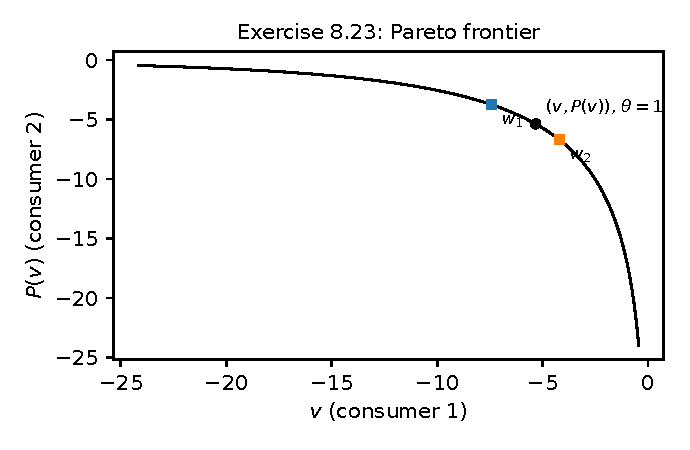
\includegraphics[width=.62\textwidth]{fig/ls08_pareto.pdf}
\captionof{figure}{Exercise 8.23: Pareto frontier with heterogeneous beliefs; continuation values $w_1<v<w_2$ at
$\theta=1$ ($r_1=.6<1<r_2=1.4$).}
\end{center}
\end{tcolorbox}

%----------------------------------------------------------------------
\subsection{Recovering Probabilities from Prices, and Corners Again (8.24--8.28)}
%----------------------------------------------------------------------

%------- 8.24 -------
\begin{tcolorbox}[evenbox,title={Exercise 8.24 \quad Recovering probabilities from prices}]
\begin{tcolorbox}[questionbox]
pp.~325--326. Consider a representative agent economy with an exogenous endowment of a single
consumption good governed by a two-state Markov chain with state $s_t\in\{1,2\}$ having transition matrix
$P$ with typical element $P_{ij}=\mathrm{Prob}(s_{t+1}=j|s_t=i)$. The representative consumer's endowment
$y_t$ is a time invariant function $y(s_t)>0$ of the Markov state. So is his consumption. The representative
consumer orders consumption streams by
\[
E_0\sum_{t=0}^\infty\beta^tu(c_t),
\]
where $\beta\in(0,1)$ and $u(c)=\frac{1}{1-\gamma}c^{1-\gamma}$ for $\gamma>0$. At each date $t\ge0$, there are
complete markets in $h$-step ahead Arrow securities of horizons $h=1,2$. Recall formula (8.10.3) for the
$h$-step ahead Arrow securities prices, which for convenience we repeat here
\[
Q_h(s_{t+h}|s_t)=\sum_{s_{t+1}}Q_1(s_{t+1}|s_t)Q_{h-1}(s_{t+h}|s_{t+1}).
\]

\textbf{a.} With an abuse of notation, arrange the one-period Arrow security prices into a $2\times2$ matrix $Q$
defined according to $Q_{ij}=Q(s_{t+1}=j|s_t=i)$. Then show that formula (8.10.3) can be represented as
$Q^h=QQ^{h-1}$ for $h\ge2$.

\textbf{b.} Suppose that you observe a complete set of one and two period ahead Arrow securities prices for
\emph{one} and only one state $i$. That is, you know the $i$th row of both $Q$ and $Q^2$. Show how you can
recover both rows of $Q$ from this information.

\textbf{c.} Recall that consumption of a representative consumer is a time-invariant function of the Markov
state. Find a formula for each element of $Q$ in terms of $\beta,\gamma$, the consumption rates in the two
states, and $P$.

\textbf{d.} Prove that if you know all elements of $Q$, you can infer $\beta$ and all elements of $P$ even if you
don't know $\gamma$.
\end{tcolorbox}

\textbf{Solution:}

\textbf{(a)} Let $Q_h$ be the matrix with $(Q_h)_{ij}=Q_h(j|i)$. (8.10.3) reads
$(Q_h)_{ij}=\sum_kQ_{ik}(Q_{h-1})_{kj}=(QQ_{h-1})_{ij}$. With $Q_1=Q$, induction gives $Q_h=QQ_{h-1}=Q^h$.

\textbf{(b)} Take $i=1$ ($i=2$ is symmetric). Row 1 of $Q^2$ is $Q^2_{1j}=Q_{11}Q_{1j}+Q_{12}Q_{2j}$, so
\[
Q_{2j}=\frac{Q^2_{1j}-Q_{11}Q_{1j}}{Q_{12}},\qquad j=1,2,
\]
provided $Q_{12}>0$, i.e.\ $P_{12}>0$ (state 2 is reachable from state 1).

\textbf{(c)} From (8.9.12) with $c=y$:
\[
Q_{ij}=\beta P_{ij}\Big(\frac{y(j)}{y(i)}\Big)^{-\gamma}.
\]

\textbf{(d)} Let $D=\mathrm{diag}(y(1)^{-\gamma},y(2)^{-\gamma})$. Then $Q=\beta D^{-1}PD$, so $Q$ is \emph{similar} to $\beta P$
and has the same eigenvalues. $P$ is stochastic, with eigenvalues $1$ and $P_{11}+P_{22}-1\in(-1,1)$. So $Q$ has
eigenvalues $\beta$ and $\beta(P_{11}+P_{22}-1)$, and
\[
\beta=\text{the largest (Perron) eigenvalue of }Q=\tfrac12\Big[\tr Q+\sqrt{(\tr Q)^2-4\det Q}\Big].
\]
Its eigenvector: $Q(D^{-1}\mathbf 1)=\beta D^{-1}P\mathbf 1=\beta D^{-1}\mathbf 1$, so $z\propto D^{-1}\mathbf 1=(y(1)^\gamma,y(2)^\gamma)'$.
The Perron vector is unique up to scale. Then $P=\beta^{-1}DQD^{-1}$, i.e.
\[
P_{ij}=\frac{Q_{ij}\,z_j}{\beta\,z_i},
\]
which uses only ratios $z_j/z_i=(y(j)/y(i))^\gamma$, which the eigenvector reveals. We never need $\gamma$ (nor the
$y$'s) separately. This is Ross's recovery theorem in a two-state economy.

\begin{tcolorbox}[databox]
$\beta=.95$, $\gamma=3$, $y=(1,1.1)$, $P=\begin{bmatrix}.9&.1\\.4&.6\end{bmatrix}$:
$Q=\begin{bmatrix}.855&.071375\\.505780&.570\end{bmatrix}$. The Perron recovery returns $\beta=.95$ and $P$ exactly,
with $z_2/z_1=1.1^3$; (b) recovers row 2 from row 1 of $Q$ and $Q^2$.
\end{tcolorbox}
\end{tcolorbox}

%------- 8.25 -------
\begin{tcolorbox}[oddbox,title={Exercise 8.25 \quad Recovering probabilities from prices, II}]
\begin{tcolorbox}[questionbox]
pp.~326--327. Consider a representative agent economy with an exogenous endowment of a single
consumption good whose geometric growth rate is governed by a two-state Markov chain with state
$s_t\in\{1,2\}$ having transition matrix $P$ with typical element $P_{ij}=\mathrm{Prob}(s_{t+1}=j|s_t=i)$. The
growth rate of the consumer's endowment $y_t$ is a time invariant function $\lambda(s_t)>0$ of the Markov state.
The endowment obeys $y_{t+1}=\lambda_{t+1}y_t$ for $t\ge0$. The representative consumer orders consumption
streams by $E_0\sum_{t=0}^\infty\beta^tu(c_t)$, where $\beta\in(0,1)$ and $u(c)=\frac{1}{1-\gamma}c^{1-\gamma}$ for $\gamma>0$.
There are complete markets in one and two period Arrow securities.

\textbf{a.} With an abuse of notation, arrange the one-period Arrow security prices into a $2\times2$ matrix $Q$
defined according to $Q_{ij}=Q(s_{t+1}=j|s_t=i)$. Then show that formula (8.10.3) can be represented as
$Q^h=QQ^{h-1}$ for $h\ge2$.

\textbf{b.} Suppose that you observe all one and two period Arrow securities prices for a single state $i$.
That is, you know the $i$th row of both $Q$ and $Q^2$. Show how you can recover both rows of $Q$ from this
information.

\textbf{c.} Find a formula for each element of $Q$ in terms of $\beta,\gamma$, and $P$.

\textbf{d.} Prove that if you know all elements of $Q$, you \emph{cannot} infer $\beta$ and all elements of $P$ even
if you know $\gamma$.
\end{tcolorbox}

\textbf{Solution:}

\textbf{(a)--(b)} Identical to 8.24(a)--(b): these steps use only (8.10.3).

\textbf{(c)} $u'(c_{t+1})/u'(c_t)=\lambda(s_{t+1})^{-\gamma}$, so
\[
Q_{ij}=\beta P_{ij}\lambda(j)^{-\gamma},\qquad Q=\beta P\Lambda,\ \ \Lambda=\mathrm{diag}(\lambda(1)^{-\gamma},\lambda(2)^{-\gamma}).
\]
(The formula also needs the growth rates $\lambda(j)$.)

\textbf{(d)} \emph{Reading:} the growth rates $\lambda(s)$ are unknown to the observer (if they were known, $\beta$
would equal the common row sum of $Q\Lambda^{-1}$, since $P\mathbf1=\mathbf1$). Since $P\mathbf 1=\mathbf 1$,
$Q(\beta\Lambda)^{-1}\mathbf 1=\mathbf 1$, so $x\equiv Q^{-1}\mathbf 1$ satisfies $x_j=1/(\beta\lambda(j)^{-\gamma})$ and
$P=Q\,\mathrm{diag}(x)$. Thus $P$ and the \emph{products} $\beta\lambda(j)^{-\gamma}$ are identified, but $\beta$ is not.
For any $\beta'\in(0,1)$ set $\lambda'(j)^{-\gamma}=1/(\beta'x_j)$. Then $\beta'P\Lambda'=Q\,\mathrm{diag}(x)\,\mathrm{diag}(1/x)=Q$:
the same prices. Knowing $\gamma$ does not help, because only $\lambda(j)^{-\gamma}$ enters. Contrast with 8.24: there
$Q=\beta D^{-1}PD$ is a \emph{similarity}, so scaling $D$ leaves $Q$ unchanged and $\beta$ is the Perron root. Here
$\Lambda$ multiplies only on the right, so a common scale of $\Lambda$ is absorbed by $\beta$. (Strictly, the statement's
claim ``cannot infer $\beta$ and all elements of $P$'' is true because of $\beta$; $P$ itself is identified.)

\begin{tcolorbox}[databox]
$\beta=.95$, $\gamma=2$, $\bar\lambda=(.97,1.03)$, $P=\begin{bmatrix}.8&.2\\.1&.9\end{bmatrix}$: $Q\,\mathrm{diag}(Q^{-1}\mathbf1)=P$
exactly. $\beta'=.90$ with $\lambda'=(.944129,1.002528)$, and $\beta'=.99$ with $\lambda'=(.990211,1.051461)$, reproduce $Q$
to machine precision.
\end{tcolorbox}
\end{tcolorbox}

%------- 8.26 -------
\begin{tcolorbox}[evenbox,title={Exercise 8.26 \quad Recovering probabilities from prices, III}]
\begin{tcolorbox}[questionbox]
p.~327. Consider a representative agent economy with an exogenous endowment of a single consumption good
governed by a two-state Markov chain with state $s_t\in\{1,2\}$ having transition matrix $P$ with typical
element $P_{ij}=\mathrm{Prob}(s_{t+1}=j|s_t=i)$. The representative consumer's endowment $y_t$ is a time invariant
function $y(s_t)>0$ of the Markov state. So is his consumption $c_t=c(s_t)$. The representative consumer
orders consumption streams by $E_0\sum_{t=0}^\infty\beta^tu(c_t)$, where $\beta\in(0,1)$, $u(c)=\frac1{1-\gamma}c^{1-\gamma}$
for $\gamma>0$, and $E_0$ denotes a mathematical expectation conditioned on date 0 information, in this case the
time 0 value $s_0$ of the state. At each date $t\ge0$, there are complete markets in one-step ahead Arrow
securities. There are also markets in $h$-period risk-free pure discount bonds. A risk-free pure discount
$h$-period bond issued at $t$ promises to pay one unit of consumption at date $t+h$ for sure. At time $t$, the
equilibrium price of a sure claim on one unit of consumption at time $t+h$ is $p^t_{t+h}$.

\textbf{a.} Please present a formula for a stochastic discount factor for pricing $h$-period ahead risky claims
for this economy. Is this stochastic discount factor unique?

\textbf{b.} Please find formulas for the equilibrium price $p^t_{t+h}$ of $h$-period risk-free pure discount bonds
for $h\ge1$.

\textbf{c.} At a single date $t$, you observe the state of the economy $s_t$. You also observe $p^t_{t+h}$ for
$h=1,2,3,4$. Your friend tells you that from these four observations you can infer $\beta,P_{11},P_{22}$, and
$\big(\frac{c(1)}{c(2)}\big)^{-\gamma}$ for this economy. Do you agree? Provide an argument.
\end{tcolorbox}

\textbf{Solution:}

Let $\kappa=(c(1)/c(2))^{-\gamma}$. Then $Q=\beta\begin{bmatrix}P_{11}&P_{12}\kappa^{-1}\\P_{21}\kappa&P_{22}\end{bmatrix}$.

\textbf{(a)} $m_{t,t+h}=\beta^h\big(c(s_{t+h})/c(s_t)\big)^{-\gamma}$. A claim paying $x(s_{t+h})$ costs
$E_t[m_{t,t+h}x]=\sum_jQ^h_{s_tj}x(j)$. Given the probability measure $P$ and complete Arrow markets, the SDF is
\emph{unique}: $m(j|i)=Q^h_{ij}/(P^h)_{ij}$ is pinned down by the Arrow prices. The decomposition is not unique,
though. For any other transition matrix $\tilde P$ with the same zero pattern, $\tilde m=Q^h_{ij}/(\tilde P^h)_{ij}$ prices every
claim identically. Prices reveal $Q$, i.e.\ probability times SDF, not the two factors separately.

\textbf{(b)} $p^t_{t+h}=\sum_jQ^h_{s_tj}=e_{s_t}'Q^h\mathbf 1$. E.g.\ $p^t_{t+1}=\beta(P_{11}+P_{12}/\kappa)$ if $s_t=1$.

\textbf{(c)} \textbf{No.} By Cayley--Hamilton, $Q^2=\tau Q-\delta I$ with $\tau=\tr Q$ and $\delta=\det Q$. So the bond prices
$p_h\equiv p^t_{t+h}$ (with $p_0=1$) satisfy
\[
p_{h+2}=\tau p_{h+1}-\delta p_h,\qquad h\ge0 .
\]
Three of these relations involve $p_1,\dots,p_4$. The first two determine $(\tau,\delta)$, provided $p_2\ne p_1^2$, and
the third is then automatically satisfied: $p_4$ carries \emph{no} new information. The data amount to three numbers,
$(p_1,\tau,\delta)$, for four unknowns. The diagonal of $Q$ has no $\kappa$, and in $\det Q$ the $\kappa$'s cancel:
\[
\tau=\beta(P_{11}+P_{22}),\qquad\delta=\beta^2(P_{11}P_{22}-P_{12}P_{21})=\beta^2(P_{11}+P_{22}-1).
\]
So $\beta$ solves $\beta^2-\tau\beta+\delta=0$: it is the larger root (the Perron root, as in 8.24), and $\sigma=P_{11}+P_{22}=\tau/\beta$
follows. The remaining datum, $p_1=\beta(P_{11}+(1-P_{11})/\kappa)$ at $s_t=1$, is one equation in the two unknowns
$(P_{11},\kappa)$ (with $P_{22}=\sigma-P_{11}$): a one-dimensional family of observationally equivalent economies.
One can infer $\beta$ and $P_{11}+P_{22}$, but not $P_{11}$, $P_{22}$ and $\kappa$ separately. Compare 8.28: there the
two-period \emph{Arrow} prices add the missing state-contingent information.

\begin{tcolorbox}[databox]
$\beta=.95$, $P_{11}=.9$, $P_{22}=.6$, $\kappa=1.2$ at $s_t=1$: $p=(.934167,\ .879937,\ .832368,\ .789053)$. The recursion holds;
$(\tau,\delta)$ from $p_1,p_2,p_3$ give $\beta=.95$. The economy with $P_{11}=.8$, $P_{22}=.7$, $\kappa=1.090909$ produces
the same four prices.
\end{tcolorbox}
\end{tcolorbox}

%------- 8.27 -------
\begin{tcolorbox}[oddbox,title={Exercise 8.27 \quad Corners}]
\begin{tcolorbox}[questionbox]
pp.~328--329. Consider an economy with exogenous endowments governed by a Markov chain with matrix
$P=\begin{bmatrix}\lambda&(1-\lambda)\\1-\delta&\delta\end{bmatrix}$ that governs transitions of a state
$s_t\in\{\bar s_1,\bar s_2\}$, where $\lambda\in(0,1),\delta\in(0,1)$. The initial probability distribution of $s_0$ is
$\pi_0$. The Markov chain induces a sequence $\{\pi_t(s^t)\}_{t=0}^\infty$ of distributions over histories
$s^t=[s_t,s_{t-1},\dots,s_0]$. There are equal numbers of two types of consumers. A consumer of type $i$ receives
an exogenous endowment $y^i(s_t)\ge0$ of a nonstorable consumption good at time, Markov state $t,s_t$.
Consumers of type 1 order consumption streams of the one good according to
\[
V_1=\sum_{t=0}^\infty\sum_{s^t}\beta^tc^1_t(s^t)\pi_t(s^t)
\]
and consumers of type 2 order consumption streams according to
\[
V_2=\sum_{t=0}^\infty\sum_{s^t}\beta^t\ln(c^2_t(s^t))\pi_t(s^t)
\]
where $c^i_t(s^t)\ge0$ is the consumption of a type $i$ consumer and $\beta\in(0,1)$ is a common discount factor.
Please note the nonnegativity constraint on consumption of each person (the force of this is that $c^i_t$ is
\emph{consumption}, not \emph{production}). The consumption good is tradable but nonstorable. There are equal
numbers of the two types of consumer.

\textbf{a.} A Pareto planner chooses a consumption allocation to maximize the criterion
$\alpha V_1+(1-\alpha)V_2$, where $\alpha\in(0,1)$. Maximization is subject to the feasibility restrictions
$\sum_ic^i_t(s^t)\le\sum_iy^i(s_t)$ for all $t\ge0$ for all $s^t$. Please characterize a Pareto optimal allocation and
get as far as you can in computing it. Under what circumstances is the constraint $c^i_t(s^t)\ge0$ binding?
When it is binding, how is the optimal allocation related to the aggregate endowment $y^1(s_t)+y^2(s_t)$?

\textbf{b.} Please define a competitive equilibrium with trading each period $t\ge0$ at each history $s^t$ of a
complete set of Arrow one-period-ahead state-contingent securities, being careful to include descriptions of
all objects that comprise a competitive equilibrium.

\textbf{c.} Compute all objects that comprise a competitive equilibrium with trading each period $t\ge0$ at each
history $s^t$ of a complete set of Arrow one-period-ahead state-contingent securities under the following
alternative auxiliary assumptions:

\textbf{Auxiliary Assumption 1:} The equilibrium allocation is such that the restrictions $c^i_t(s^t)\ge0$ never
bind for any $i$.

\textbf{Auxiliary Assumption 2:} The equilibrium allocation is such that the restrictions $c^i_t(s^t)\ge0$ always
bind for some $i$.
\end{tcolorbox}

\textbf{Solution:}

Write $Y(s)=y^1(s)+y^2(s)$.

\textbf{(a)} With multipliers $\zeta_t(s^t)$ on feasibility, the Kuhn--Tucker conditions are
\[
\alpha\beta^t\pi_t\le\zeta_t\ \ (=\text{ if }c^1_t>0),\qquad(1-\alpha)\beta^t\pi_t/c^2_t=\zeta_t .
\]
If $c^1_t>0$, then $\zeta_t=\alpha\beta^t\pi_t$ and $c^2_t=(1-\alpha)/\alpha$. Type 2 never hits zero (Inada). Hence
\[
\boxed{c^2_t(s^t)=\min\Big\{Y(s_t),\frac{1-\alpha}{\alpha}\Big\},\qquad c^1_t(s^t)=\max\Big\{Y(s_t)-\frac{1-\alpha}{\alpha},\,0\Big\}.}
\]
The allocation depends only on $s_t$. Type 1's constraint binds iff $Y(s_t)<(1-\alpha)/\alpha$, i.e.\ in low-endowment
states or when type 1's weight is small. Then type 2 consumes the whole aggregate endowment, $c^2=Y(s_t)$, and
consumer 2's consumption moves one-for-one with $Y$. Otherwise type 2 is fully insured at $(1-\alpha)/\alpha$ and the
risk-neutral type 1 absorbs all fluctuations.

\textbf{(b)} Objects: a kernel $Q(s'|s)$; natural debt limits $\bar A^i(s)=y^i(s)+\sum_{s'}Q(s'|s)\bar A^i(s')$; value
functions $v^i(a,s)$; decision rules $c=h^i(a,s)$, $\hat a(s')=g^i(a,s,s')$; initial wealths $a^i_0=0$. Given $Q$
and $\bar A^i$, $v^i$ solves
$v^i(a,s)=\max\{u_i(c)+\beta\sum_{s'}v^i(\hat a(s'),s')P(s'|s)\}$ s.t.\ $c+\sum_{s'}Q(s'|s)\hat a(s')\le y^i(s)+a$,
\textbf{$c\ge0$}, $-\hat a(s')\le\bar A^i(s')$, with $u_1(c)=c$ and $u_2=\ln$. Markets clear: $c^1+c^2=Y(s)$ and
$\hat a^1(s')+\hat a^2(s')=0$.

\textbf{(c)} \emph{General solution.} Type 2 is always interior, so $Q(s'|s)=\beta P(s'|s)c^2(s)/c^2(s')$. Type 1's
marginal value of wealth $\varphi(s)=\partial v^1/\partial a$ satisfies $\varphi(s)\ge1$, with equality where
$c^1(s)>0$ (FOC for $c$), and the Euler equation $Q(s'|s)\varphi(s)=\beta P(s'|s)\varphi(s')$. Both hold with
$\varphi(s)=\bar c/c^2(s)$ and
\[
c^2(s)=\min\{Y(s),\bar c\},\qquad c^1(s)=Y(s)-c^2(s).
\]
$\bar c$ comes from type 2's budget with $a^2_0=0$. Time-0 prices implied by $Q$ are $q^0_t=\beta^t\pi_tc^2(s_0)/c^2(s_t)$,
so the value of $c^2$ is $c^2(s_0)/(1-\beta)$ and the value of $y^2$ is $c^2(s_0)\sum_t\beta^tE_{s_0}[y^2/c^2]$:
\[
e_{s_0}'(I-\beta P)^{-1}\Big[\frac{y^2(s)}{\min\{Y(s),\bar c\}}\Big]_s=\frac{1}{1-\beta}. \tag{$\dagger$}
\]
The left side is decreasing in $\bar c$, so $\bar c$ is unique. Holdings $\hat a^i(s)=\Upsilon^i(s)=[(I-Q)^{-1}(c^i-y^i)](s)$
and debt limits $\bar A^i=(I-Q)^{-1}y^i$ complete the equilibrium. The Pareto weight is $\alpha=1/(1+\bar c)$.

\emph{Assumption 1 (never binds).} $\varphi\equiv1$, so $Q=\beta P$; $c^2=\bar c$ constant, and ($\dagger$) gives
$\bar c=(1-\beta)e_{s_0}'(I-\beta P)^{-1}y^2$, the annuity value of type 2's endowment. $c^1(s)=Y(s)-\bar c$, which requires
$\bar c<\min_sY(s)$. Type 2 is perfectly insured by the risk-neutral type 1 at actuarially fair prices.

\emph{Assumption 2 (binds).} Only type 1 can be at the corner. \emph{Reading:} ``always bind'' cannot mean
$c^1\equiv0$ in every state, since type 1 would then never spend a positive wealth. It means the constraint binds
in the low-endowment state $\bar s_1$ whenever it occurs, and not in $\bar s_2$ (so $Y(\bar s_1)\le\bar c<Y(\bar s_2)$). Then
$c^1(\bar s_1)=0$, $c^2(\bar s_1)=Y(\bar s_1)$, $c^2(\bar s_2)=\bar c$, $\varphi(\bar s_1)=\bar c/Y(\bar s_1)\ge1$, and
\[
Q=\beta\begin{bmatrix}\lambda&(1-\lambda)Y(\bar s_1)/\bar c\\(1-\delta)\,\bar c/Y(\bar s_1)&\delta\end{bmatrix},\qquad
\bar c=\frac{m_2\,y^2(\bar s_2)}{\frac{1}{1-\beta}-m_1\,y^2(\bar s_1)/Y(\bar s_1)},
\]
where $(m_1,m_2)=e_{s_0}'(I-\beta P)^{-1}$. Claims paying in the corner state are expensive. Type 1 values wealth
there at $\varphi>1$, and the kernel is no longer $\beta P$.

\begin{tcolorbox}[databox]
Illustration $\lambda=.8$, $\delta=.6$, $\beta=.9$, $s_0=\bar s_1$. \emph{Case A} (Assumption 1): $y^1=(1,1.5)$,
$y^2=(.5,.3)$: $\bar c=.44375$ ($\alpha=.6926$), $Q=\beta P$, $\Upsilon^1=(0,-.3125)$, $\bar A^1=(11.406,12.188)$,
$\bar A^2=(4.4375,4.125)$. \emph{Case B} (Assumption 2): $y^1=(.05,1.5)$, $y^2=(.3,1)$: $\bar c=.732558$
($\alpha=.5772$), $c^1=(0,1.767442)$, $c^2=(.35,.732558)$, $\varphi=(2.093,1)$,
$Q=\begin{bmatrix}.72&.086\\.753488&.54\end{bmatrix}$, $\Upsilon^1=(0,.581395)$. Both cases: Arrow budgets of both
types hold in every state, type 1's Euler equation with $\varphi$ holds, and the KKT signs are right.
\end{tcolorbox}
\end{tcolorbox}

%------- 8.28 -------
\begin{tcolorbox}[evenbox,title={Exercise 8.28 \quad Recovering probabilities from prices, IV}]
\begin{tcolorbox}[questionbox]
pp.~329--330. Consider an economy with an exogenous endowment governed by a Markov chain with transition
matrix $P=\begin{bmatrix}\lambda&(1-\lambda)\\1-\delta&\delta\end{bmatrix}$ that governs transitions of a state
$s_t\in\{\bar s_1,\bar s_2\}$, where $\lambda\in(0,1),\delta\in(0,1)$. The initial distribution over $s_0$ is $\pi_0$. The
Markov chain induces a sequence $\{\pi_t(s^t)\}_{t=0}^\infty$ of distributions over histories
$s^t=[s_t,s_{t-1},\dots,s_0]$. There is a representative consumer who orders consumption plans according to
\[
\sum_{t=0}^\infty\sum_{s^t}\beta^tu(c_t(s^t))\pi_t(s^t)
\]
where $u(c)=(1-\gamma)^{-1}c^{1-\gamma}$ and $\gamma>0$ and $\beta\in(0,1)$. There is one consumer called the
representative consumer. The representative consumer's endowment is $y_t=\bar y_1>0$ if $s_t=\bar s_1$ and
$y_t=\bar y_2>0$ if $s_t=\bar s_2$.

\textbf{a.} Define a competitive equilibrium with trading at each date, history pair $t,s^t$ of one-period-ahead
Arrow state contingent securities. Please define all components of a competitive equilibrium, including the
allocation and the price system.

\textbf{b.} Show that equilibrium one-period Arrow state-contingent security prices can be arranged into a
$(2\times2)$ matrix $Q^{(1)}$ whose $(i,j)$ component $Q^{(1)}_{i,j}$ is the price of one unit of consumption when
Markov state $s_{t+1}=\bar s_j$ tomorrow when the Markov state $s_t$ today is in state $\bar s_i$. Please give
formulas for all elements of $Q^{(1)}$ in terms of the fundamental parameters of the economy
$\beta,\gamma,\lambda,\delta,\bar y_1,\bar y_2$.

\textbf{c.} Define a competitive equilibrium with trading at each date, history pair $t,s^t$ of both
one-period-ahead and two-period-ahead Arrow state contingent securities. Let two-period Arrow
state-contingent security prices be arranged into a $(2\times2)$ matrix $Q^{(2)}$ whose $(i,j)$ component
$Q^{(2)}_{i,j}$ is the price of one unit of consumption when Markov state $s_{t+2}=\bar s_j$ two periods ahead
when the Markov state $s_t$ today is in state $\bar s_i$. Please give formulas for all elements of $Q^{(2)}$ in
terms of the fundamental parameters of the economy $\beta,\gamma,\lambda,\delta,\bar y_1,\bar y_2$.

\textbf{d.} (``inverse problem'') An outsider observes this economy. The outsider knows the theoretical
structure of the economy but does not know the parameter values $[\lambda,\delta,\beta,\gamma,\bar y_1,\bar y_2]$. But at
a particular date at which $s_t=\bar s_1$, the outsider observes
\[
[Q^{(1)}(1,1),Q^{(1)}(1,2),Q^{(2)}(1,1),Q^{(2)}(1,2)].
\]
Please interpret these observations. From these observations alone, can the outsider infer $\lambda,\delta,\beta$?
Please explain your answer.
\end{tcolorbox}

\textbf{Solution:}

\textbf{(a)} A kernel $Q(s'|s)$, natural debt limits $\bar A(s)$, a value function $v(a,s)$, decision rules
$c=h(a,s)$, $\hat a(s')=g(a,s,s')$, and $a_0=0$. Given $Q$ and $\bar A$, these solve the consumer's Bellman
equation (8.9.8)--(8.9.10), and markets clear: $c=y(s)$, $\hat a(s')=0$. The allocation is $c_t=y(s_t)$.

\textbf{(b)} From (8.9.12), $Q^{(1)}_{ij}=\beta P_{ij}(\bar y_j/\bar y_i)^{-\gamma}$. With $\kappa\equiv(\bar y_2/\bar y_1)^{-\gamma}$:
\[
Q^{(1)}=\beta\begin{bmatrix}\lambda&(1-\lambda)\kappa\\(1-\delta)/\kappa&\delta\end{bmatrix}.
\]

\textbf{(c)} With both markets, the budget is (8.10.1) with $j\le2$. The equilibrium adds the two-period prices, the
allocation is still $c=y$, and by (8.10.3) $Q^{(2)}=Q^{(1)}Q^{(1)}$:
\[
Q^{(2)}_{11}=\beta^2[\lambda^2+(1-\lambda)(1-\delta)],\quad Q^{(2)}_{12}=\beta^2(1-\lambda)(\lambda+\delta)\kappa,
\]
\[
Q^{(2)}_{21}=\beta^2(1-\delta)(\lambda+\delta)/\kappa,\quad Q^{(2)}_{22}=\beta^2[\delta^2+(1-\lambda)(1-\delta)].
\]
(For example, $Q^{(2)}_{12}=\beta\lambda\cdot\beta(1-\lambda)\kappa+\beta(1-\lambda)\kappa\cdot\beta\delta$.)

\textbf{(d)} \emph{Interpretation.} Standing in $\bar s_1$, the four numbers are the prices of one unit of
consumption delivered next period if the state is $\bar s_1$ / $\bar s_2$, and two periods ahead if the state is
$\bar s_1$ / $\bar s_2$. Their row sums are the one- and two-period risk-free bond prices. \emph{Inference: yes, for
$\lambda,\delta,\beta$} (and $\kappa$, though not $\gamma$, $\bar y_1$, $\bar y_2$ separately). Let
$a=Q^{(1)}_{11}$, $b=Q^{(1)}_{12}$, $c=Q^{(2)}_{11}$, $d=Q^{(2)}_{12}$. Then:
\[
a=\beta\lambda,\qquad\frac db=\beta(\lambda+\delta)\ \Rightarrow\ e\equiv\frac db-a=\beta\delta,
\]
\[
c=\beta^2\lambda^2+(\beta-\beta\lambda)(\beta-\beta\delta)=a^2+(\beta-a)(\beta-e).
\]
So $\beta$ solves $\beta^2-(a+e)\beta+ae-(c-a^2)=0$. Since $c-a^2=\beta^2(1-\lambda)(1-\delta)>0$, one root exceeds
$\max(a,e)$ and the other lies below $\min(a,e)$. $\beta$ must exceed both $a=\beta\lambda$ and $e=\beta\delta$, so it is the
larger root:
\[
\beta=\frac{(a+e)+\sqrt{(a-e)^2+4(c-a^2)}}{2},\qquad\lambda=\frac a\beta,\qquad\delta=\frac e\beta,\qquad
\kappa=\frac{b}{\beta(1-\lambda)} .
\]
This is 8.24(b) (row recovery) followed by 8.24(d) (Perron root), done by hand. Contrast 8.26: risk-free bond
prices alone are not enough.

\begin{tcolorbox}[databox]
$\lambda=.85$, $\delta=.7$, $\beta=.96$, $\gamma=2$, $\bar y=(1,1.2)$: observations $(.816,\ .1,\ .707328,\ .1488)$. Then
$e=.672$, roots $.96$ and $.528$, and the recovered values are $\beta=.96$, $\lambda=.85$, $\delta=.7$,
$\kappa=.694444=1.2^{-2}$. The Perron root of the full $Q^{(1)}$ is also $.96$.
\end{tcolorbox}
\end{tcolorbox}

%======================================================================
\section*{Companion code}
\addcontentsline{toc}{section}{Companion code}
%======================================================================

Every numerical result above is reproduced by the notebook \texttt{ls\_ch08.ipynb} in this folder
(executed, outputs saved). Each claim is checked by an independent route with an \texttt{assert}.

\begin{center}
\begin{tabular}{@{}lp{11.2cm}@{}}
\toprule
\textbf{Section} & \textbf{What it checks} \\
\midrule
Shared & Markov helpers: kernel $\beta P_{ij}\mu_j/\mu_i$, (8.10.3) by explicit double sum, history enumeration, stationary distribution. The ch.~5/7 LQ toolkit is not needed (no LQ problem here). \\
8.1--8.3 & Closed forms vs SLSQP; $\partial W/\partial s=\theta$; decentralised consumers; $v_\theta'$ and $v_\theta''$ by finite differences. \\
8.4--8.7 & Matrix prices vs enumeration of all histories; $(I-K)^{-1}$ vs truncated series; $Q^h$ vs (8.10.3); Arrow budgets with $a=\Upsilon$. \\
8.8 & Tax smoothing: closed form vs SLSQP over state-contingent revenue; government budget in both states. \\
8.9--8.10 & Budgets and KKT conditions on 4000 periods; interest rates; sequential budgets. \\
8.11--8.13 & $\tilde\pi$ sums to one; three representations of $a_0$; early-resolution holdings and debt limits. \\
8.14 & Shares by inverse vs truncated sum; bond spanning; alternation closed form; default region (closed form vs utility sums; figure). \\
8.15--8.19 & \texttt{brentq} on budgets; Euler equations of both consumers; binding natural debt limits. \\
8.20--8.23 & Risk-free rates; entropy inequality; simulated beliefs selection (figure); recursive Pareto by binomial sums vs FOCs and envelope (figure). \\
8.24--8.28 & Perron recovery; non-identification families (8.25, 8.26); corner equilibria in a Markov economy; quadratic-in-$\beta$ recovery. \\
\bottomrule
\end{tabular}
\end{center}

Figures are saved to \texttt{fig/ls08\_*.pdf} with TrueType (not Type~3) fonts.

\end{document}
